\documentclass{article}

% Use NeurIPS style for clean formatting with preprint footer
\usepackage[preprint]{neurips_2024}
\usepackage[utf8]{inputenc}
\usepackage[T1]{fontenc}
\usepackage[hidelinks]{hyperref}
\usepackage{url}
\usepackage{booktabs}
\usepackage{amsfonts}
\usepackage{amsmath}
\usepackage{amssymb}
\usepackage{nicefrac}
\usepackage{microtype}
\usepackage{graphicx}
\usepackage{subcaption}
\usepackage{algorithm}
\usepackage{algorithmic}
\usepackage{natbib}
\usepackage{placeins}  % \FloatBarrier — keeps floats within their section

\title{Recovering Sparse Neural Connectivity from Partial Measurements:\\
A Covariance-Based Approach with Granger-Inspired Refinement}

\author{
  Quilee Simeon \\
  Massachusetts Institute of Technology \\
  \texttt{qsimeon@mit.edu}
}

\begin{document}

\maketitle

\begin{abstract}
Inferring the connectivity of neural circuits from incomplete observations is a fundamental challenge in neuroscience: imaging field-of-view, sparse indicator expression, and restricted optical access typically limit each recording to a different random subset of neurons, so the experimentalist sees a circuit through many partial windows rather than one complete view.
We ask whether the connectivity of a recurrent network can nevertheless be recovered by combining these windows.
Our approach is to accumulate pairwise covariance statistics across sessions wherever two neurons happen to be co-observed, then perform a single global pseudoinverse rather than inverting each session separately---a design choice we show is what makes recovery possible at all.
A Granger-inspired refinement step enforces biological constraints (no autapses, non-negative weights, lagged-covariance sparsity) by projected gradient descent.
A central and counterintuitive finding emerges: a linear estimator that ignores the network's nonlinearity \emph{outperforms} an oracle estimator that knows it, because the oracle's compressed covariance is worse-conditioned---a concrete biological instance of James--Stein shrinkage.
Systematic experiments characterize a control--estimation tradeoff (stimulation aids identifiability but disrupts the intrinsic dynamics that make the circuit biologically meaningful) and an error decomposition showing that drive from intrinsic circuit oscillators, not nonlinearity mismatch, is the dominant remaining bottleneck.
\end{abstract}

\begin{figure}[!t]
\centering
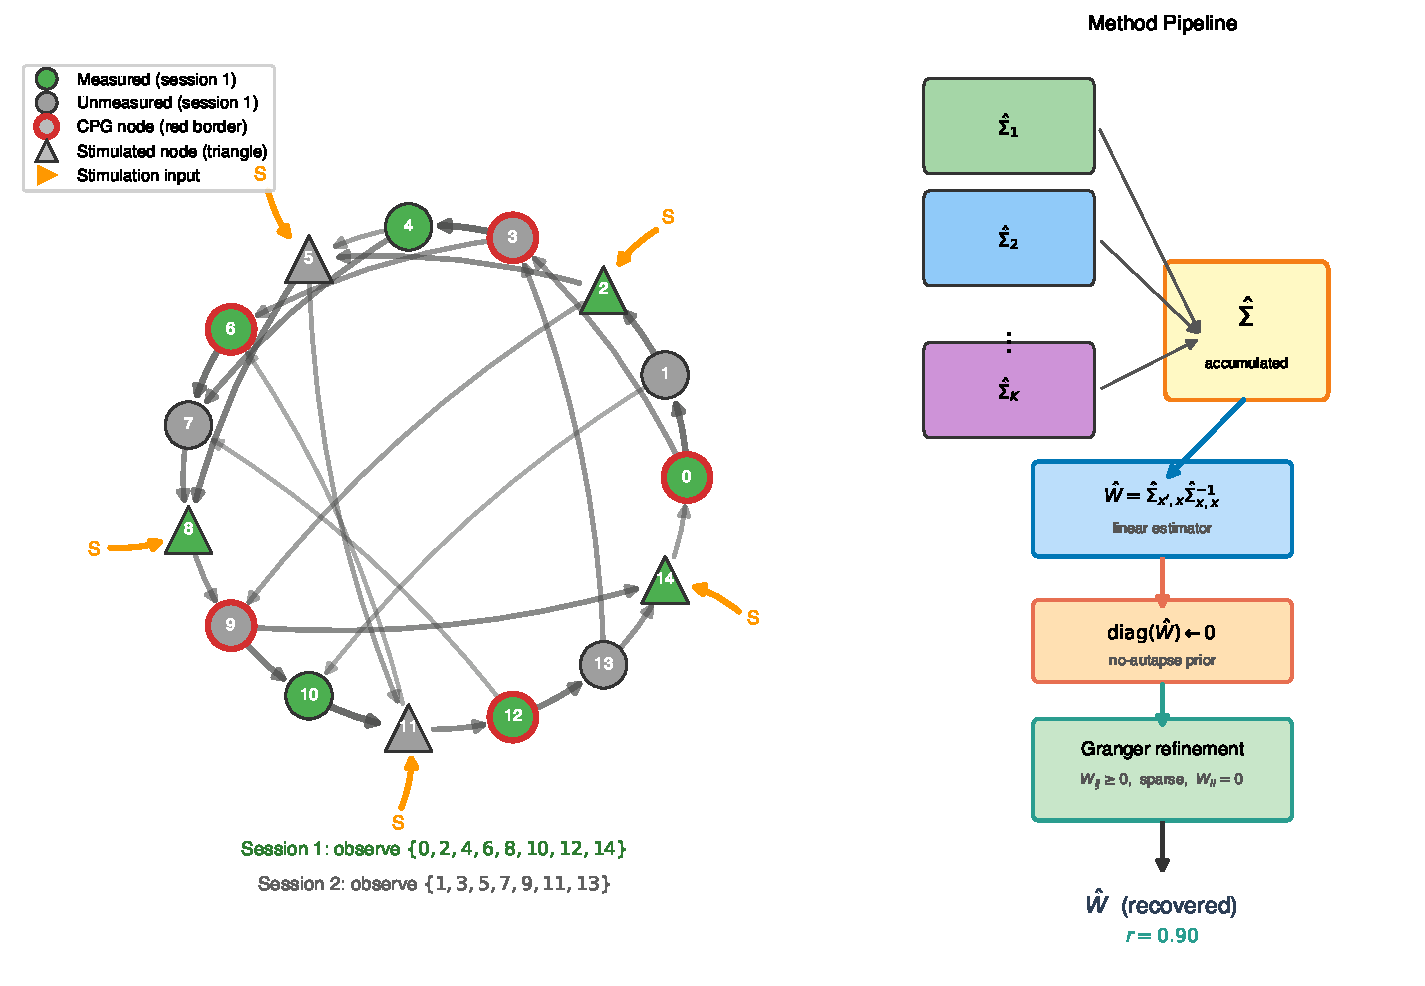
\includegraphics[width=\linewidth]{figures/fig1_problem_schematic.pdf}
\caption{\textbf{Problem setup and estimation pipeline.} \textbf{(Left)} A network of $N=15$ neurons with directed weighted connectivity $W$. In a given session, a subset of neurons (green) is measured while the rest (gray) are unobserved. Red-bordered nodes are CPG drivers (intrinsic oscillatory input); triangle nodes receive extrinsic stimulation (orange arrows ``S''). \textbf{(Right)} The method pipeline: each of $K$ sessions yields a partial covariance matrix $\hat{\Sigma}_k$ covering only co-observed neuron pairs. These are accumulated element-wise into $\hat{\Sigma}$, from which $W$ is estimated via least-squares inversion, the diagonal is zeroed (no-autapse prior), and the result is refined by projected gradient descent enforcing a Granger-inspired lagged-covariance sparsity constraint.}
\label{fig:schematic}
\end{figure}

% ============================================================================
\section{Introduction}
\label{sec:intro}
% ============================================================================

A central goal in systems neuroscience is to map the connectivity of neural circuits from functional measurements \citep{power2011functional}.
Small neural circuits, from the lobster stomatogastric ganglion (${\sim}30$ neurons; \citep{marder2007understanding}) and \textit{C.~elegans} (302 neurons; \citep{white1986structure, cook2019whole}) to larval zebrafish \citep{ahrens2013whole} and cortical organoids \citep{quadrato2017cell}, span tens to thousands of neurons and serve as tractable model systems for studying circuit function. In each case, even cutting-edge whole-brain functional imaging rarely captures the entire circuit simultaneously: limited field of view, sparse indicator expression, and restricted optical access mean that what one actually accumulates over a campaign is a stack of overlapping but never-complete partial recordings.
This creates a fundamental inverse problem: given partial, noisy measurements of neural dynamics across multiple sessions---and assuming, as an idealization, that the underlying connectivity does not drift between them---can we recover the full connectivity matrix? More abstractly, this is a partial-window instance of the broader system-identification problem of recovering a recurrent dynamical system from sub-sampled observations, with neuroscience as the most pressing case.

This problem embodies a \emph{control-estimation tradeoff} related to classical notions of persistent excitation in system identification \citep{ljung1998system}: stimulating neurons with random perturbations aids connectivity estimation by exciting network modes, but disrupts the intrinsic dynamics that make the circuit biologically relevant.
Experimentalists must balance identifiability against preservation of natural dynamics.
Furthermore, real circuits possess intrinsic oscillatory patterns, specifically central pattern generators (CPGs) \citep{marder2001central}, whose detailed structure is unknown to the experimenter.
These represent \emph{unmodeled autonomous dynamics} that influence the observed activity.

We formalize this as a matrix recovery problem from partial observations.
Consider a network of $N$ neurons with connectivity matrix $W \in \mathbb{R}^{N \times N}$, governed by discrete-time recurrent dynamics \citep{sussillo2009generating}, where $W_{ij}$ represents the synaptic weight from neuron $j$ to neuron $i$.
In each recording session, we observe a subset of neurons and stimulate a (possibly different) subset.
Our key insight is that pairwise covariance statistics can be accumulated across sessions: whenever neurons $i$ and $j$ are simultaneously observed, their covariance contributes to estimating the $(i,j)$ block of $W$.

\paragraph{Contributions.}
Our central design choice is to pool pairwise covariances across sessions \emph{before} matrix inversion---a single global solve rather than per-session inversions averaged together. This choice yields four results:
\begin{itemize}
    \item We derive a covariance-based estimator $\hat{W} = \Sigma_{x_{t+1},x_t} \Sigma_{x_t,x_t}^{-1}$ for connectivity recovery from partial measurements and provide identifiability conditions.
    \item We introduce a Granger-inspired \citep{granger1969investigating} sparsity refinement via projected gradient descent that enforces a lagged-covariance non-causality criterion, complementing structural priors (no autapses, non-negativity) applied uniformly to all estimates.
    \item We discover an \emph{implicit regularization} effect: the ``incorrect'' linear approximation yields a better-conditioned estimator than the oracle with known nonlinearity, analogous to James--Stein shrinkage \citep{james1961estimation}.
    \item We systematically characterize the tradeoff between stimulation strength and measurement density, revealing that optimal stimulation depends on the fraction of observed neurons.
\end{itemize}

% ============================================================================
\section{Problem Formulation}
\label{sec:formulation}
% ============================================================================

\subsection{Dynamical System Model}

We model the neural circuit as a discrete-time recurrent dynamical system:
\begin{equation}
    x_{t+1} = W \phi(x_t) + b_t
    \label{eq:dynamics}
\end{equation}
where $x_t \in \mathbb{R}^N$ is the neural state, $W \in \mathbb{R}^{N \times N}$ is the connectivity matrix, $\phi: \mathbb{R} \to \mathbb{R}$ is an element-wise nonlinearity, and $b_t \in \mathbb{R}^N$ is the total input comprising both extrinsic stimulation and intrinsic central pattern generator (CPG) drive.
This arises from discretizing a continuous-time neural circuit $\tau \, d\mathbf{x}/dt = -\tilde{M} \phi(\mathbf{x}) + \tilde{\mathbf{b}}$ with time constant $\tau$ and coupling matrix $\tilde{M}$, yielding $W = I - (\Delta t / \tau)\tilde{M}$.

\paragraph{Modeling priors on network topology and weights.}
We impose three structural priors on $W$, each a modeling choice motivated by practical and mathematical considerations:

\emph{(i) No autapses}: $W_{ii} = 0$ for all $i$. Self-connections are not reported as distinct structural features in connectomics reconstructions of \textit{C.~elegans} \citep{white1986structure, cook2019whole} or \textit{Drosophila}, and in a strongly connected graph, a self-loop on neuron $i$ is approximated by indirect paths $i \to j \to i$. Operationally, we zero the diagonal of $\hat{W}$ before any refinement. This is an architectural belief, qualitatively distinct from the oracle's biophysical knowledge of $\phi$ (E6).

\emph{(ii) Strong connectivity}: We require the digraph to be strongly connected, ensuring that for any node $i$ and any stimulated set $\mathcal{S}$, there exists a directed path from some $s \in \mathcal{S}$ to $i$.
This is a practical requirement for identifiability: in a weakly connected graph, sink components receive no stimulation signal, leaving their covariance rows rank-deficient (see Appendix~\ref{sec:app_connectivity}).
Empirically, weakly connected topologies produced dead zones where activity collapsed to zero, while strong connectivity ensured signal reverberation through the entire network.
This prior is consistent with the recurrent interneuron cores of biological circuits: a large fraction of neurons in the \textit{Drosophila} whole-brain connectome lie in a giant strongly connected component \citep{lin2024network}, and central pattern generators rely on reciprocal connectivity to sustain rhythmic output \citep{marder2007understanding}.
Sensory input and motor output neurons typically sit outside this recurrent core \citep{varshney2011structural}, so the strong-connectivity prior is best understood as a model of the \emph{processing} stage of a circuit rather than a full sensory-to-motor pipeline.

\emph{(iii) Non-negative weights}: $W_{ij} \geq 0$.
Like the no-autapse prior, this is a modeling belief applied uniformly to \emph{all} estimates (both the raw covariance estimator and the Granger-refined output), not a constraint specific to any refinement step.
It is motivated by the measurement modality: EM connectomics, the primary source of ground-truth wiring data, measures synapse \emph{size} (contact area, vesicle count) but not synapse \emph{sign} (excitatory vs.\ inhibitory), yielding an inherently unsigned weight matrix.
In our formulation, inhibitory effects arise from the \emph{sign of the activity}: a positive weight applied to negative (hyperpolarized) presynaptic activity drives the postsynaptic neuron downward.
This is a dual of the standard neuroscience convention (non-negative firing rates with signed weights), and is functionally equivalent for the covariance estimator, which assumes no sign structure on $W$.
By the Perron--Frobenius theorem, non-negative irreducible matrices have a unique maximal real eigenvalue with a positive eigenvector, which simplifies spectral radius control and ensures stable dynamics.
The method generalizes to mixed-sign weights (see Section~\ref{sec:discussion}).

\paragraph{Nonlinearity.}
We require the element-wise nonlinearity $\phi$ to be \emph{1-Lipschitz}: $|\phi'(x)| \leq 1$ for all $x$.
Combined with $\rho(W) \leq 1$, this guarantees contractivity of the autonomous dynamics.
Our default is $\phi = \tanh$, which is 1-Lipschitz, bounded, and odd-symmetric ($\tanh(-x) = -\tanh(x)$, so $\tanh(0) = 0$); these additional properties enable exact error analysis via the Stein--Price identity (Section~\ref{sec:methods}).
To assess robustness, we test three additional nonlinearities in E5 (Section~\ref{sec:experiments}):
\emph{identity} ($\phi(x) = x$, 1-Lipschitz but unbounded),
\emph{ReLU} ($\phi(x) = \max(0, x)$, 1-Lipschitz but neither odd nor bounded), and
\emph{sigmoid} ($\phi(x) = 1/(1+e^{-x})$, 1-Lipschitz and bounded but not odd, with $\phi(0) = 0.5 \neq 0$).
This deliberately includes nonlinearities that violate our default's symmetry and boundedness, testing how gracefully the estimator degrades.

\paragraph{Stability.}
For stability, we require $\rho(W) \leq 1$, where $\rho(\cdot)$ denotes the spectral radius.
Combined with the 1-Lipschitz property of $\phi$, this ensures bounded autonomous dynamics ($b_t = 0$): since $\|\phi(x)\| \leq \|x\|$ and $\rho(W) \leq 1$, the map $x \mapsto W\phi(x)$ is non-expansive.
The spectral radius is scaled to $\rho(W) \approx 1.0$ (edge of stability), producing marginally stable dynamics that are neither trivially decaying nor divergent.
With $\rho(W) \leq 1$ and 1-Lipschitz $\phi$ satisfying $|\phi(x)| < |x|$ for $x \neq 0$ (as with $\tanh$), the autonomous system ($b_t = 0$) \emph{contracts to the origin}: the network falls silent without input.
This motivates the central pattern generator (CPG) component of the input $b_t$: a subset of neurons possess autonomous oscillatory drive (analogous to cardiac pacemaker cells) that sustains network activity in the absence of external stimulation \citep{marder2001central}.
The input thus decomposes as $b_t = b_t^{\text{stim}} + b_t^{\text{CPG}}$, where $b_t^{\text{stim}}$ is extrinsic i.i.d.\ Gaussian noise (independent of $x_t$) and $b_t^{\text{CPG}} = \text{cpg}(x_t)$ is state-dependent intrinsic drive with $\text{Cov}(b_t^{\text{CPG}}, x_t) \neq 0$.
This decomposition is critical: the extrinsic component satisfies our independence assumption, while the CPG component violates it and dominates the estimation error (Section~\ref{sec:discussion}).

\emph{CPG identity is hidden from the estimation pipeline.}
Which neurons possess intrinsic drive is a property of the ground-truth simulation, not available to the observer.
In each session, any measured or stimulated node may also be a CPG node; the experimenter does not know.
The variance-based CPG detection described in Section~\ref{sec:discussion} is a \emph{post-hoc} analysis, not an oracle input to the estimator.
This mirrors the biological reality: a real experimenter typically cannot identify pacemaker neurons \emph{a priori}.

\subsection{Observation Model}

In session $k$, we observe a subset $\mathcal{M}_k \subseteq \{1, \ldots, N\}$ of neurons and stimulate a subset $\mathcal{S}_k$.
The observed activity is:
\begin{equation}
    y_t^{(k)} = P_{\mathcal{M}_k} x_t + \epsilon_t, \qquad \epsilon_t \sim \mathcal{N}(0, \sigma_\epsilon^2 I)
\end{equation}
where $P_{\mathcal{M}_k}$ is a projection onto the observed neurons and $\epsilon_t$ is i.i.d.\ measurement noise.
Our experiments test both noiseless ($\sigma_\epsilon = 0$) and noisy ($\sigma_\epsilon > 0$) regimes; the method is robust to moderate noise (Section~\ref{sec:discussion}).

\subsection{The Estimation Problem}

Given $K$ sessions with observations $\{y_t^{(k)}\}_{t=1}^{T_k}$ for $k = 1, \ldots, K$, recover $W$.

% ============================================================================
\section{Methods}
\label{sec:methods}
% ============================================================================

\subsection{Covariance-Based Estimator}

Under the linear approximation $\phi(x) \approx x$ (valid when $\|x\|$ is small), Eq.~\eqref{eq:dynamics} simplifies to $x_{t+1} \approx W x_t + b_t$.
Assuming statistical independence between inputs $b_t$ and states $x_t$ (an approximation we revisit critically in Section~\ref{sec:discussion}), the cross-covariance of the \emph{true} states satisfies:
\begin{equation}
    \Sigma_{x_{t+1}, x_t} = W \Sigma_{x_t, x_t} + \underbrace{\Sigma_{b_t, x_t}}_{\approx 0}
    \label{eq:covariance}
\end{equation}

In the noiseless case ($\sigma_\epsilon = 0$, so $y_t = x_t$), this directly yields the estimator $\hat{W} = \Sigma_{y_{t+1}, y_t} \Sigma_{y_t, y_t}^{-1}$.
When observation noise is present ($\sigma_\epsilon > 0$), the observed covariances differ from the true state covariances.
Since $\epsilon_t$ is i.i.d.\ and independent of $x_t$:
\begin{align}
    \Sigma_{y_t, y_t} &= \Sigma_{x_t, x_t} + \sigma_\epsilon^2 I \label{eq:noisy_cov} \\
    \Sigma_{y_{t+1}, y_t} &= \Sigma_{x_{t+1}, x_t} \quad \text{(noise at $t{+}1$ independent of $y_t$)}
\end{align}
The estimator computed from observed data is therefore:
\begin{equation}
    \hat{W} = \Sigma_{y_{t+1}, y_t} \bigl(\Sigma_{y_t, y_t}\bigr)^{-1} = W \Sigma_{x,x} \bigl(\Sigma_{x,x} + \sigma_\epsilon^2 I\bigr)^{-1}
    \label{eq:estimator}
\end{equation}
This is a \emph{ridge-regularized} version of the true $W$: observation noise shrinks the estimate toward zero, with $\sigma_\epsilon^2$ playing the role of the ridge parameter.
For small noise ($\sigma_\epsilon \ll \sigma_{\min}(\Sigma_{x,x})$), the effect is negligible; for large noise, the estimate is over-regularized.

\paragraph{No-autapse prior.}
Before any further refinement, we enforce the structural prior $\hat{W}_{ii} = 0$ for all $i$.
This is a case of the experimenter applying a \emph{modeling belief} about the underlying circuit (namely, that autapses are absent), and this belief happens to be correct because we constructed the ground truth this way.
The diagonal of the raw estimate $\hat{\Sigma}_{y_{t+1},y_t} \hat{\Sigma}_{y_t,y_t}^{-1}$ is dominated by single-neuron autocorrelation ($3$--$4\times$ larger than off-diagonal entries; see Figure~\ref{fig:granger}A), which does not reflect genuine self-connectivity.
Zeroing the diagonal removes this artifact and is the single most impactful step in the pipeline: in ablation experiments (E2, Section~\ref{sec:experiments}), it accounts for the majority of the improvement over the chance baseline.
Note that this prior is qualitatively different from the oracle knowledge tested in E6: it is a structural assumption about circuit architecture, whereas E6 tests knowledge of the neuronal transfer function $\phi$, a biophysical property that would require single-cell measurements to determine.

\paragraph{Accumulation across sessions.}
For each pair $(i,j)$, we compute empirical covariances from the \emph{observed} data $y_t$ only in sessions where both neurons $i$ and $j$ are simultaneously measured.
Let $S_{ij}^{(k)} = \mathbf{1}[i \in \mathcal{M}_k \wedge j \in \mathcal{M}_k]$ indicate co-measurement.
The accumulated covariance is:
\begin{equation}
    \hat{\Sigma}_{ij} = \frac{\sum_{k=1}^{K} S_{ij}^{(k)} \hat{\Sigma}_{ij}^{(k)}}{\sum_{k=1}^{K} S_{ij}^{(k)}}
\end{equation}
where $\hat{\Sigma}_{ij}^{(k)}$ is the empirical covariance of the observed $y_t$ from session $k$.

\paragraph{Error analysis.}
The estimation error decomposes into two terms:
\begin{equation}
    \hat{W} - W = \underbrace{W\bigl[\Sigma_{\phi(x),x} - \Sigma_{x,x}\bigr]\Sigma_{x,x}^{-1}}_{e_1:\text{ model mismatch}} + \underbrace{\Sigma_{b,x}\Sigma_{x,x}^{-1}}_{e_2:\text{ input correlation}}
    \label{eq:error}
\end{equation}
The first term, $e_1$, captures the price of treating $\phi$ as the identity; the second, $e_2$, captures the violation of the standard input-state independence assumption when the drive $b_t$ is correlated with the state.
For $\phi = \tanh$ and Gaussian states, both terms admit a closed form via the Stein--Price identity (Appendix~\ref{sec:app_price}): $\Sigma_{\phi(x),x} = D \Sigma_{x,x}$ for a diagonal $D \in (0,1)^{N\times N}$, so $e_1 = W(D-I)$ scales with the state variance and is $O(\sigma^2)$ in the small-noise regime---substantially tighter than generic Lipschitz bounds.
Both error sources are amplified by $\|\Sigma_{x,x}^{-1}\|_2$, so ill-conditioned covariance (from sparse measurement) degrades recovery even when the model is correct.

\subsection{Granger-Inspired Sparsity Refinement}
\label{sec:granger}

The raw estimator $\hat{W}$ already enforces the structural priors from Section~\ref{sec:formulation}: no autapses ($\hat{W}_{ii} = 0$) and non-negativity ($W_{ij} \geq 0$).
We add one further sparsity constraint, inspired by the intuition behind Granger causality~\citep{granger1969investigating}: if neuron $j$'s present value is \emph{more} correlated with neuron $i$'s present than with $i$'s future, then $j$ carries no additional predictive signal about $i$'s next state beyond what their shared context already explains, so the directed edge $j \to i$ can be zeroed.

\textbf{Granger non-causality rule}: set $W_{ij} = 0$ wherever
\begin{equation}
    \hat{\Sigma}_{x_t, x_t}(i,j) \;>\; \hat{\Sigma}_{x_{t+1}, x_t}(i,j),
    \label{eq:granger_rule}
\end{equation}
i.e., wherever the lag-0 (contemporaneous) covariance exceeds the lag-1 (future-on-past) covariance.
This captures the core intuition of Granger causality---``future informativeness beyond present informativeness''---applied as a deterministic threshold on pooled covariance entries rather than as a classical F-test on residual variances.
Two caveats: (i)~the rule is a \emph{necessary} (not sufficient) condition for $W_{ij} = 0$, and (ii)~it is one-sided and therefore relies on the non-negativity prior $W_{ij} \geq 0$; a negative edge could reduce the lag-1 covariance relative to the lag-0 and satisfy the inequality falsely.
We formalize the derivation and discuss failure modes in Appendix~\ref{sec:app_granger_rule}.

The rule is enforced as a projection inside a least-squares refinement, rather than as a standalone edge-selection test.
We solve
\begin{equation}
    \min_A \|A - \hat{\Sigma}_{x_{t+1}, x_t}\|_F^2 \quad \text{s.t.} \quad A \hat{\Sigma}_{x_t, x_t}^{-1} \in \mathcal{C}
    \label{eq:optimization}
\end{equation}
where $\mathcal{C}$ is the intersection of four constraint sets: zero diagonal, non-negativity, spectral-radius bound, and the Granger-inspired zero-mask from Eq.~\eqref{eq:granger_rule}.
By optimizing over $A = W\hat{\Sigma}_{x_t,x_t}$ rather than $W$ directly, the objective becomes a Frobenius distance to the observed cross-covariance, while constraints are enforced on $W = A\hat{\Sigma}_{x_t,x_t}^{-1}$ via projection.
Iterating a trust-region step on $A$ with projection onto $\mathcal{C}$ yields a refined estimator that is the Frobenius-closest feasible point to the raw covariance-based solution.

\subsection{Full Pipeline}

The complete method is summarized in Algorithm~\ref{alg:pipeline} and illustrated in Figure~\ref{fig:schematic}.

\begin{algorithm}[ht]
\caption{Covariance Accumulation + Granger-Inspired Refinement}
\label{alg:pipeline}
\begin{algorithmic}[1]
\REQUIRE Sessions $\{(y_t^{(k)}, \mathcal{M}_k)\}_{k=1}^K$
\ENSURE Estimated connectivity $\hat{W}$
\STATE Initialize $\hat{\Sigma}_{y_{t+1},y_t} \leftarrow 0$, $\hat{\Sigma}_{y_t,y_t} \leftarrow 0$, $C \leftarrow 0$ \COMMENT{accumulators}
\FOR{$k = 1, \ldots, K$}
    \STATE Compute session covariances from observed data $\{y_t^{(k)}\}_{t=1}^{T_k}$
    \STATE $S \leftarrow \mathbf{1}_{\mathcal{M}_k} \mathbf{1}_{\mathcal{M}_k}^T$ \COMMENT{co-measurement mask}
    \STATE $\hat{\Sigma}_{y_{t+1},y_t} \mathrel{+}= S \odot \hat{\Sigma}^{(k)}_{y_{t+1},y_t}$; \quad $\hat{\Sigma}_{y_t,y_t} \mathrel{+}= S \odot \hat{\Sigma}^{(k)}_{y_t,y_t}$
    \STATE $C \mathrel{+}= S$
\ENDFOR
\STATE $\hat{\Sigma}_{y_{t+1},y_t} \leftarrow \hat{\Sigma}_{y_{t+1},y_t} \oslash C$; \quad $\hat{\Sigma}_{y_t,y_t} \leftarrow \hat{\Sigma}_{y_t,y_t} \oslash C$ \COMMENT{average}
\STATE $\hat{W}_{\text{approx}} \leftarrow \hat{\Sigma}_{y_{t+1},y_t} \cdot \hat{\Sigma}_{y_t,y_t}^{\dagger}$ \COMMENT{pseudoinverse handles rank-deficient $\hat{\Sigma}$; Eq.~\eqref{eq:estimator}}
\STATE $\text{diag}(\hat{W}_{\text{approx}}) \leftarrow 0$; \quad $\hat{W}_{\text{approx}} \leftarrow \max(\hat{W}_{\text{approx}}, 0)$ (element-wise) \COMMENT{structural priors: no autapses, non-negativity}
\STATE $\hat{W} \leftarrow \text{GrangerRefine}(\hat{W}_{\text{approx}}, \hat{\Sigma}_{y_t,y_t}, \hat{\Sigma}_{y_{t+1},y_t}, \mathcal{C})$ \COMMENT{Granger-inspired sparsity, Eq.~\eqref{eq:optimization}}
\RETURN $\hat{W}$
\end{algorithmic}
\end{algorithm}

We evaluate this pipeline on synthetic networks designed to capture key properties of small biological circuits, varying network size, session duration, stimulation protocol, and nonlinearity.
Each experiment isolates one factor while holding the others fixed, so that the resulting effects can be attributed unambiguously.
The experimental setup and baselines are described next.

% ============================================================================
\section{Experiments}
\label{sec:experiments}
% ============================================================================

\subsection{Experimental Setup}

We generate synthetic networks modeling neural circuits at biologically motivated scales:
\begin{itemize}
    \item Random directed graphs with non-negative weights and spectral radius $\rho(W) \leq 1$
    \item Intrinsic dynamics driven by central pattern generators (CPGs) modeled as chaotic reservoir networks
    \item Extrinsic stimulation as \emph{independent} i.i.d.\ Gaussian noise applied to each stimulated node at each timestep (the most favorable case for identifiability; correlated or shared stimulation would reduce the rank of the input covariance)
\end{itemize}

Each node in the network is characterized by three (non-exclusive) Boolean roles: whether it is a \emph{CPG node} (receives autonomous intrinsic drive), a \emph{stimulated node} (receives extrinsic stimulation), and a \emph{measured node} (its activity is recorded).
These roles are assigned randomly per session, modeling the experimental reality that different recording sessions observe and stimulate different neuron subsets.

Each experiment in Table~\ref{tab:design} is a \emph{sweep} over one parameter (two, in E3) with the remaining parameters fixed at default values.
Unless noted otherwise, the defaults are $N=15$, $T=1000$, $K=50$ sessions, 10 measured neurons, 5 stimulated, 5 CPG nodes, $\sigma=1.0$, and $\phi=\tanh$; at $N=15$, integer discretization gives $10/15 \approx 66\%$ measured and $5/15 \approx 33\%$ stimulated/CPG.
Two experiments necessarily override these defaults: E1 jointly varies $N$ and $T$, scaling $(|\mathrm{CPG}|, |\mathrm{stim}|, |\mathrm{meas}|) = (N/3, N/3, 2N/3)$ with network size; E7 fixes $N=30$ to allow a meaningful sweep over the number of stimulated neurons.
Critically, a parameter being swept in a given experiment is \emph{not} held at its default in that experiment---that sweep is precisely the object of study.
\paragraph{Sampling structure within a sweep.}
A \emph{condition} is a single fixed parameter setting within a sweep (e.g., one cell of the E1 $N{\times}T$ grid, or one value $\sigma=0.5$ in E6).
One \emph{repetition} of a condition draws a single random connectivity matrix $W$, simulates $K=50$ recording sessions sharing that $W$ (each with an independent random measurement mask $\mathcal{M}_k$ and stimulation subset $\mathcal{S}_k$), and evaluates recovery; we choose $K=50$ as a small constant that exceeds the coupon-collector pair-coverage threshold $K_{\min} \!=\! \mathcal{O}(\log N / p^2)$ across all tested $N$ at $p=2/3$ measurement (Appendix~\ref{sec:app_connectivity}).
We run 10 repetitions per condition (10 distinct random topologies) to measure variability across circuits, using bootstrap resampling for confidence intervals.
The two levels serve distinct purposes: the 50 sessions per topology are necessary for covariance accumulation; the 10 topologies give error bars over the space of possible circuits.
We report median Frobenius distance $\|W - \hat{W}\|_F / N$ with 95\% bootstrap confidence intervals ($n_{\text{resamples}}=1000$).

\paragraph{Reference baselines.}
We compare recovery error against a hierarchy of reference estimates, each incorporating strictly more ground-truth information than the last (see E2 ablation, Figure~\ref{fig:granger}H):
\begin{itemize}
    \item \emph{Chance}: a dense random draw from the same prior weight distribution used to generate $W$, $W_{\mathrm{rand}} \sim U(0,1)^{N \times N}$. Knows only that weights are non-negative; has no sparsity pattern and no spectral constraint. This is the weakest possible guess and sets the error floor.
    \item \emph{Adjacency}: the Chance draw element-wise masked by the true sparsity pattern, $W_{\mathrm{rand}} \odot \mathbf{1}[W \neq 0]$. Knows \emph{which} edges exist but not their weights or the network's spectral radius.
    \item \emph{Spectral}: the Adjacency baseline further rescaled to the true spectral radius $\rho(W)$. This baseline has everything we know about $W$ from the generative prior---sparsity pattern \emph{and} spectral radius---and is therefore an independent draw from the full prior distribution of $W$. It is the fairest ``guess from the prior alone'' comparison, because any improvement over it must come from data, not from generative knowledge.
    \item \emph{VAR}: per-session vector autoregressive baseline (single-lag OLS on each session's observed sub-network, averaged element-wise across co-observed sessions). Represents the ``invert-then-accumulate'' alternative to our global design; full definition in Appendix~\ref{sec:app_baselines}.
    \item \emph{GLM}: per-neuron ridge-regularized linear model ($\alpha=1$), fit per-session and averaged; full definition in Appendix~\ref{sec:app_baselines}. Tests whether local L2 regularization recovers the same bias-variance sweet spot as our global estimator.
    \item \emph{Estimate}: our covariance-based method (Algorithm~\ref{alg:pipeline}) with no oracle knowledge of the generative parameters.
    \item \emph{Granger}: \emph{Estimate} refined with the Granger-inspired lagged-covariance zero constraints (Section~\ref{sec:granger}).
\end{itemize}
For compactness we abbreviate these as Chance, Adj, Spec, VAR, GLM, Est, and Grn in figure panels and captions.
The primary comparison is against the \emph{Spectral} baseline: improvement from $0.120$ to $0.083$ ($31\%$), which isolates the contribution of data-driven estimation beyond what the generative prior alone provides.
As shown in Figure~\ref{fig:granger}H, the VAR achieves error $0.136$ (worse than even the Spectral prior), and the Ridge-GLM achieves $0.117$ (slightly better than Spectral due to the regularization bias, but $36\%$ worse than our estimator at $0.086$). Both confirm that pooling before the global inversion is the critical design choice.

\begin{table}[ht]
\centering
\caption{Experimental design: each experiment sweeps one or two parameters while fixing the rest at defaults (E1 scales CPG/stim/meas counts with $N$; E7 sets $N{=}30$).}
\label{tab:design}
\small
\begin{tabular}{cp{3.2cm}p{4.5cm}p{3.8cm}}
\toprule
Exp & Parameter swept & Values & Question \\
\midrule
E1 & Network size $N$, duration $T$ & $N \in \{15,159,300\}$, $T \in \{100,350,1000\}$ & How does recovery scale? \\
E2 & Method ablation & Chance $\to$ VAR $\to$ GLM $\to$ Est $\to$ Granger & What does each step add? \\
E3 & Stim gain $\times$ measurement & $\sigma \in [0,2]$, meas $\in \{33,66,100\%\}$ & Is there a stim-measurement interaction? \\
E4 & Measurement fraction & $33$--$100\%$ & How much observation is needed? \\
E5 & Nonlinearity $\phi$ & tanh, ReLU, identity, sigmoid & How robust to model mismatch? \\
E6 & Oracle vs.\ approximation & $\sigma \in [0,5]$ & Does the oracle ever win? \\
E7 & Stimulation fraction & $\{0\%, 33\%, 66\%\}$ of $N{=}30$ & How many neurons to stimulate? \\
E8 & Observation noise $\sigma_\epsilon$ & $\{0, 0.05, 0.1, 0.2, 0.5\}$ & How robust to measurement noise? \\
\bottomrule
\end{tabular}
\end{table}

The subsections below present experiments in order (E1--E8): baseline scaling (E1), Granger ablation (E2, the central pooling-vs-per-session comparison), stimulation tradeoff (E3), measurement density (E4), nonlinearity robustness (E5), oracle comparison (E6, the James--Stein finding), stimulation coverage (E7), and noise robustness (E8).

\subsection{Baseline Recovery (E1)}

Before characterising individual experimental factors in isolation, we first establish that the estimator works and ask the most basic question: how does recovery error scale with network size $N$ and recording duration $T$?
Table~\ref{tab:baseline} shows recovery error across network sizes $N \in \{15, 159, 300\}$ and recording durations $T \in \{100, 350, 1000\}$ with $66\%$ measurement.
The covariance estimator (with structural priors: no autapses, non-negativity) consistently outperforms the chance baseline.
For $N{=}15$, recovery saturates early: $T{=}350$ already achieves near-minimal error ($0.082$), with no further improvement at $T{=}1000$ ($0.083$).
For larger networks ($N \geq 159$), recovery is poor at $T{=}100$ due to covariance ill-conditioning, but improves dramatically at $T{=}350$ and beyond.
The best overall result is $N{=}300$, $T{=}1000$ (error $0.014$, $97.5\%$ improvement over chance), demonstrating that larger networks with sufficient recording time enable better recovery (Figure~\ref{fig:scaling}).

\begin{table}[ht]
\centering
\caption{Median Granger-refined recovery error (Frobenius / $N$) across network sizes and durations ($66\%$ measurement, 10 topologies, 50 sessions each). Bold indicates the best result per $N$. Chance baseline ranges from $0.555$ ($N{=}15$) to $0.576$ ($N{=}300$). For $N{=}15$, error saturates by $T{=}350$; for $N \geq 159$, $T{=}100$ yields poor recovery due to covariance ill-conditioning, but $T \geq 350$ gives excellent results. Best overall: $N{=}300$, $T{=}1000$ ($0.014$, $97.5\%$ improvement over chance).}
\label{tab:baseline}
\begin{tabular}{cccc}
\toprule
$N$ & $T{=}100$ & $T{=}350$ & $T{=}1000$ \\
\midrule
15   & 0.086 & \textbf{0.082} & 0.083 \\
159  & 0.167 & 0.022 & \textbf{0.019} \\
300  & 0.130 & 0.018 & \textbf{0.014} \\
\bottomrule
\end{tabular}
\end{table}

\begin{figure}[ht]
\centering
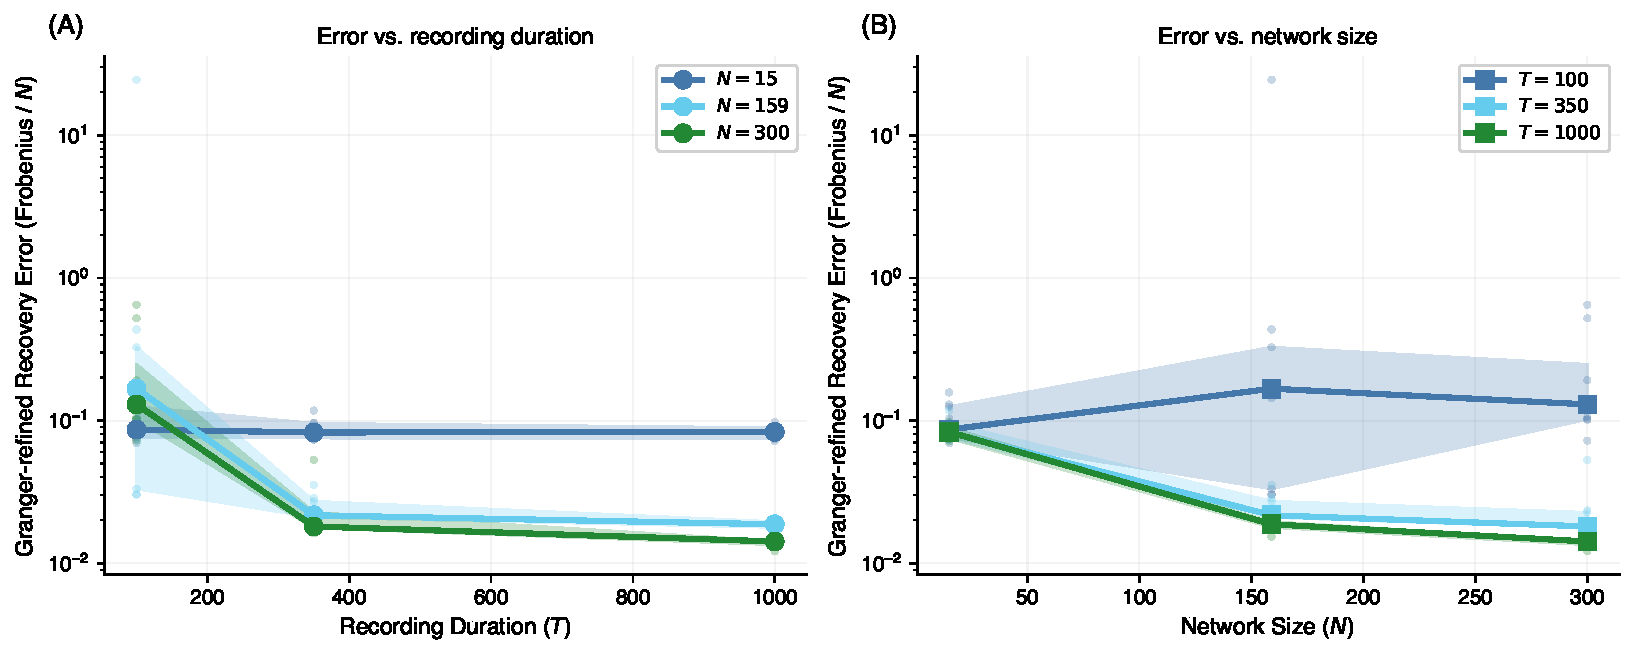
\includegraphics[width=\linewidth]{figures/fig2_scaling.pdf}
\caption{\textbf{Scaling properties of the covariance estimator.} \textbf{(A)} Median recovery error (Frobenius distance / $N$) vs.\ recording duration $T$ for three network sizes ($N \in \{15, 159, 300\}$) with $66\%$ measurement. Shaded regions show 95\% bootstrap confidence intervals over 10 random topologies (50 sessions each). For $N{=}15$, error saturates by $T{=}350$; for $N \geq 159$, covariance ill-conditioning at $T{=}100$ gives way to excellent recovery at $T \geq 350$. Best results: $N{=}300$ ($0.014$) and $N{=}159$ ($0.019$) at $T{=}1000$. \textbf{(B)} Error vs.\ network size $N$ at fixed recording durations $T \in \{100, 350, 1000\}$.}
\label{fig:scaling}
\end{figure}

\subsection{Granger-Inspired Refinement (E2)}

E2 asks what each component of the pipeline contributes and whether a simpler baseline could achieve the same recovery: can we recover well without the Granger-inspired refinement? Would a per-session VAR or Ridge-GLM be enough?
We evaluate on $N=15$ networks with $T=1000$, $66\%$ measurement, and 10 random topologies.
After enforcing the no-autapse prior ($W_{ii} = 0$) and non-negativity ($W_{ij} \geq 0$) on the raw estimate, the Granger-inspired refinement further reduces error by an additional $\sim 3\%$ through its non-causality sparsity pattern.

The raw estimate is dense (nearly all off-diagonal entries positive), yielding high recall (median $0.97$) but low precision (median $0.30$).
The Granger-inspired refinement improves precision to $0.40$ while maintaining recall at $0.96$, eliminating spurious edges without sacrificing true connectivity.
The estimator achieves a $31\%$ improvement over an independent draw from the same generative prior ($0.083$ vs.\ $0.120$), demonstrating that the covariance accumulation framework extracts genuine connectivity information beyond what structural knowledge alone provides.
The constraint that $W_{ij} = 0$ where $\Sigma_{x_t, x_t}(i,j) > \Sigma_{x_{t+1}, x_t}(i,j)$ effectively identifies non-causal pairs via the lagged-covariance criterion (Figure~\ref{fig:granger}).
Taken together, the VAR and Ridge-GLM baselines (Appendix~\ref{sec:app_baselines}) confirm that the global accumulate-then-invert design---not the Granger-inspired refinement alone---is the essential ingredient: local per-session inversions, even when regularized, trail our global estimator by $36$--$58\%$.

\begin{figure}[!tbp]
\centering
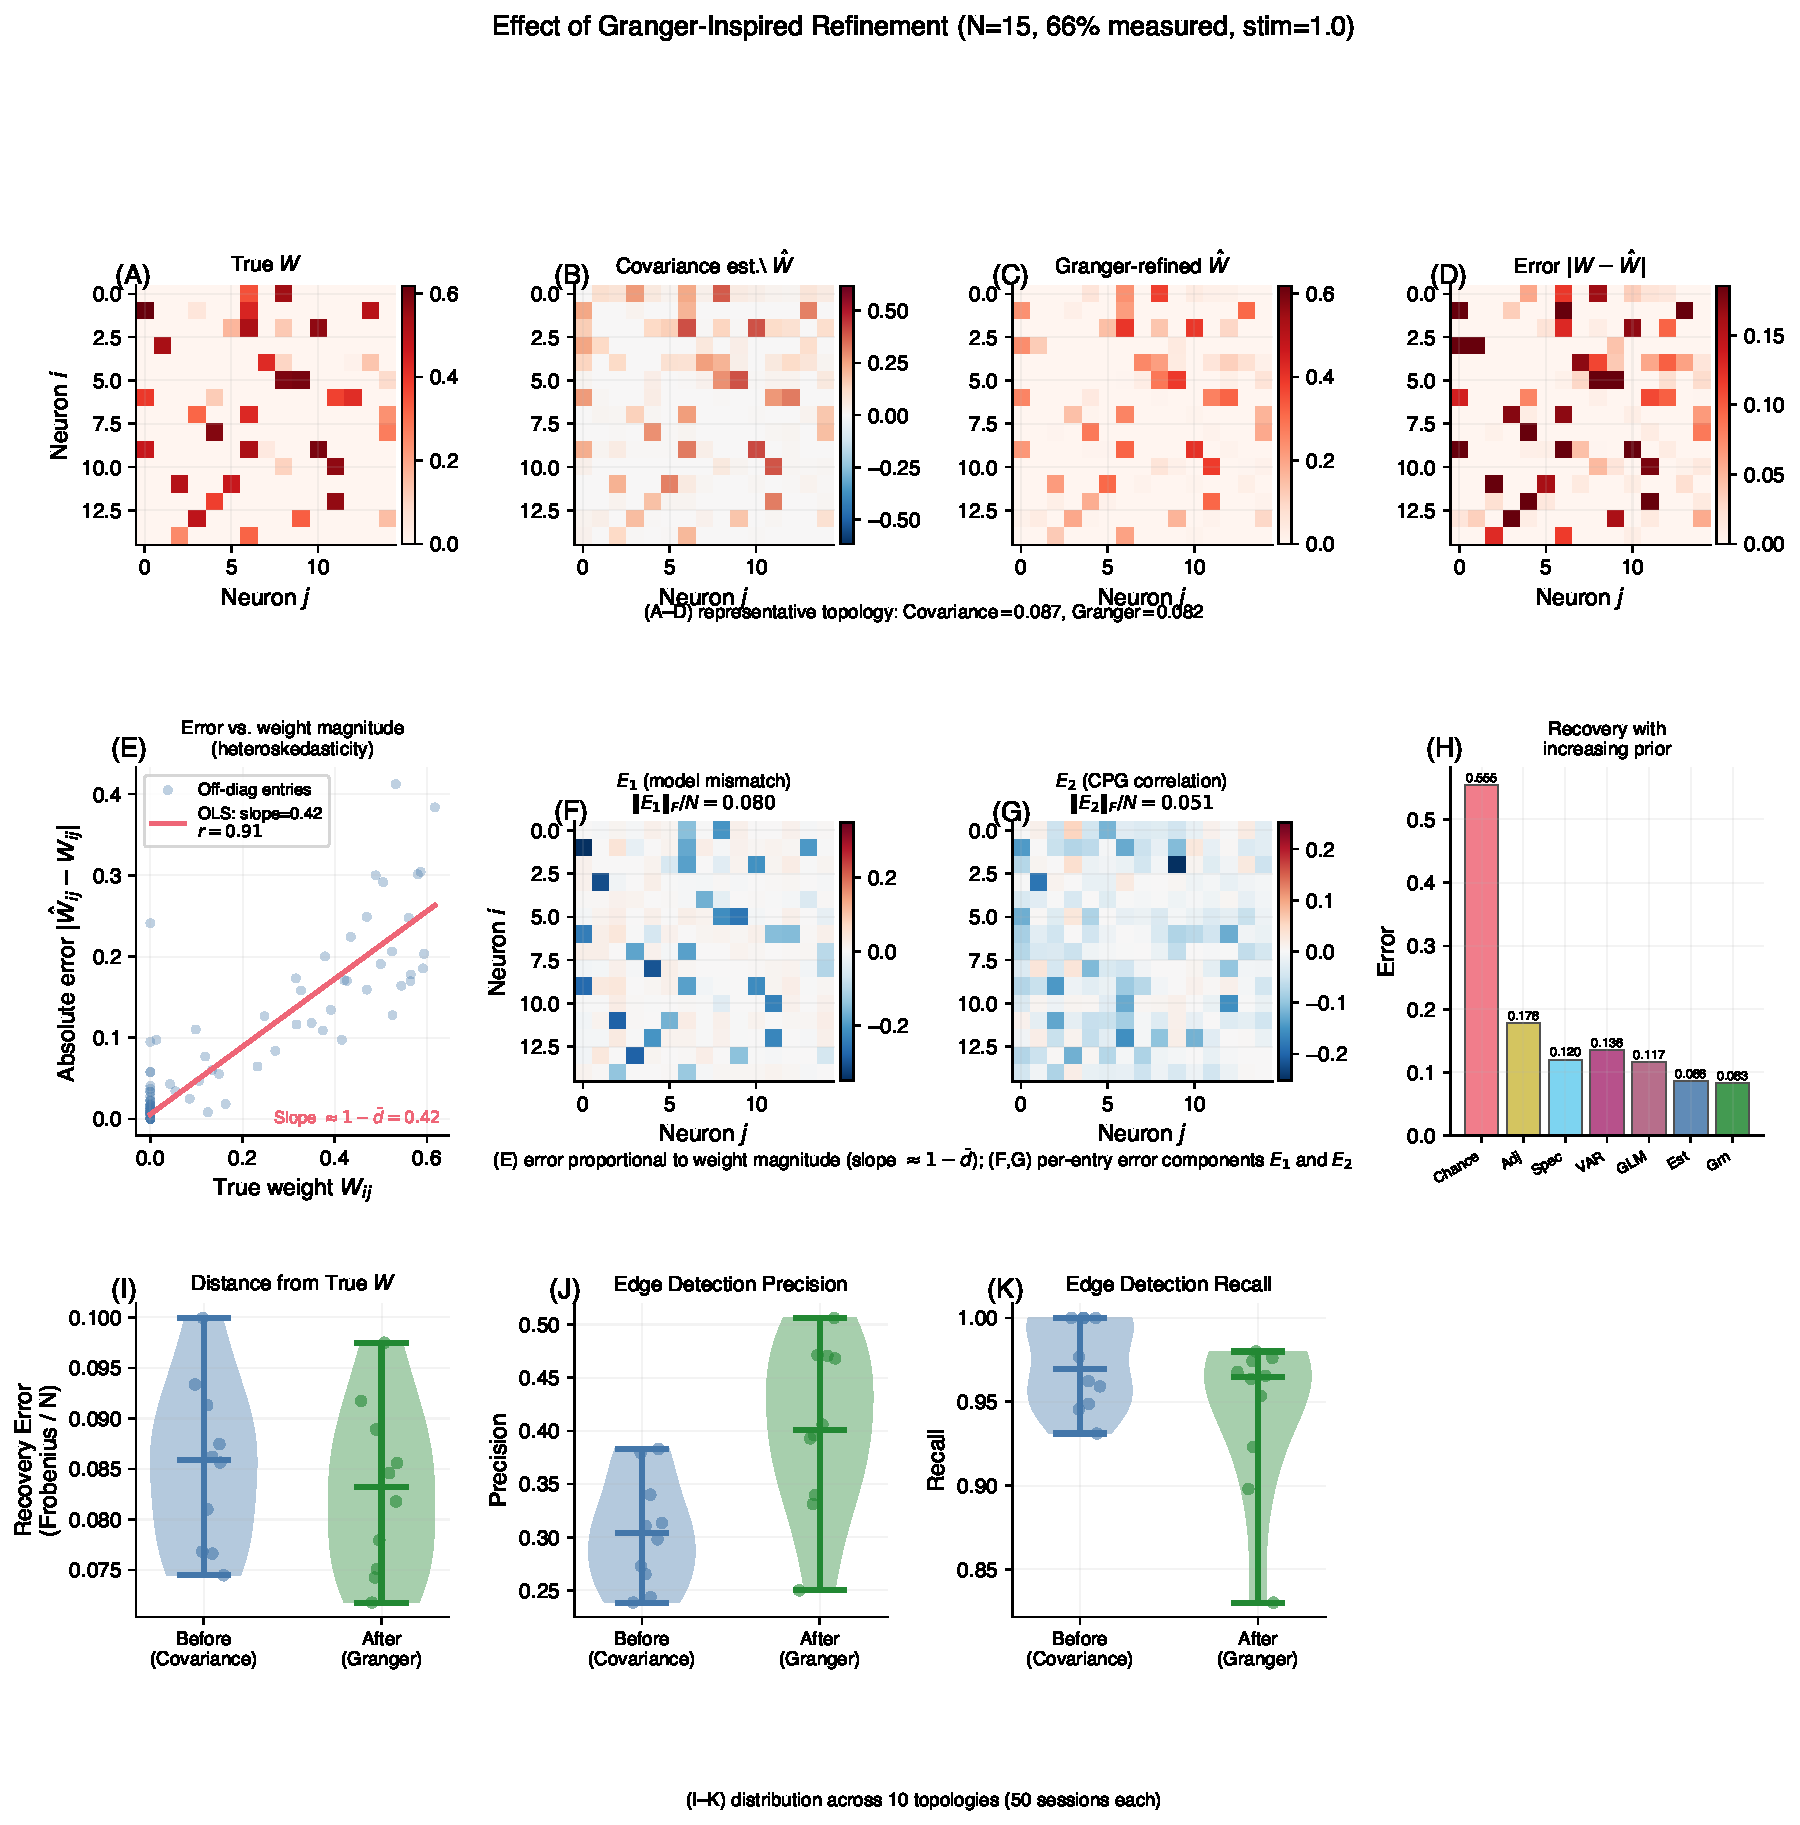
\includegraphics[width=\linewidth]{figures/fig3_granger_refinement.pdf}
\caption{\textbf{Effect of Granger-inspired refinement and error structure} ($N=15$, $66\%$ measured, $\sigma=1.0$). \textbf{(A--D)} Weight matrix heatmaps from a representative topology: (A)~true $W$, (B)~raw covariance estimate $\hat{W}$, (C)~Granger-refined $\hat{W}$, (D)~absolute error $|W-\hat{W}|$. \textbf{(E)} Error-weight scatter: each off-diagonal entry's absolute error $|\hat{W}_{ij}-W_{ij}|$ vs.\ true weight $W_{ij}$.
The positive correlation ($r\approx0.91$, OLS slope $\approx 1-\bar{d}$) reflects the heteroskedastic structure of $e_1=W(D-I)$: the estimator systematically shrinks larger weights more (see Appendix~\ref{sec:app_hetero}).
\textbf{(F)}~Per-entry $e_1$ (model mismatch) and \textbf{(G)}~$e_2$ (CPG correlation) heatmaps for the same topology; $e_2$ is ${\sim}2.8\times$ larger in Frobenius norm.
\textbf{(H)} Ablation: Chance $\to$ Adj $\to$ Spec $\to$ VAR $\to$ GLM $\to$ Est $\to$ Grn. The VAR (per-session OLS, $0.136$) is worse than even the oracle Spectral prior ($0.120$); the Ridge-GLM (per-session $\ell_2$-regularized, $0.117$) is slightly better, yet both are far worse than our accumulate-then-invert estimate ($0.086$). Granger refines further to $0.083$ ($31\%$ over Spec).
\textbf{(I--K)} Violin plots over 10 topologies: Frobenius error (I), edge precision (J, $0.30\to0.40$), edge recall (K, maintained at $0.96$).}
\label{fig:granger}
\end{figure}

\FloatBarrier
\subsection{Stimulation-Dynamics Tradeoff (E3)}

Having established that the estimator works, we now ask: how should an experimentalist choose the stimulation protocol?
We examine the interaction between stimulation gain $\sigma$ and measurement fraction for $N=15$, $T=1000$.
The results reveal a fundamental \emph{interaction effect}: the optimal stimulation level depends critically on measurement density.

At low measurement ($33\%$), recovery error is relatively insensitive to stimulation level because partial observation implicitly regularizes $\Sigma_{x,x}$.
At full measurement ($100\%$), zero stimulation yields substantially degraded recovery, while moderate stimulation ($\sigma \approx 0.5$) yields the best performance.
This occurs because CPG-driven dynamics alone do not excite all network modes; without stimulation, $\Sigma_{x,x}$ becomes ill-conditioned.
A small amount of stochastic input breaks the CPG autocorrelation structure and ensures persistent excitation.
However, beyond $\sigma \approx 1$, recovery begins to degrade as noise dominates the signal (Figure~\ref{fig:tradeoff}).

This confirms the control-estimation tradeoff: experimentalists must balance stimulation strength against signal quality, with the optimal level depending on how many neurons are simultaneously observed.

\begin{figure}[ht]
\centering
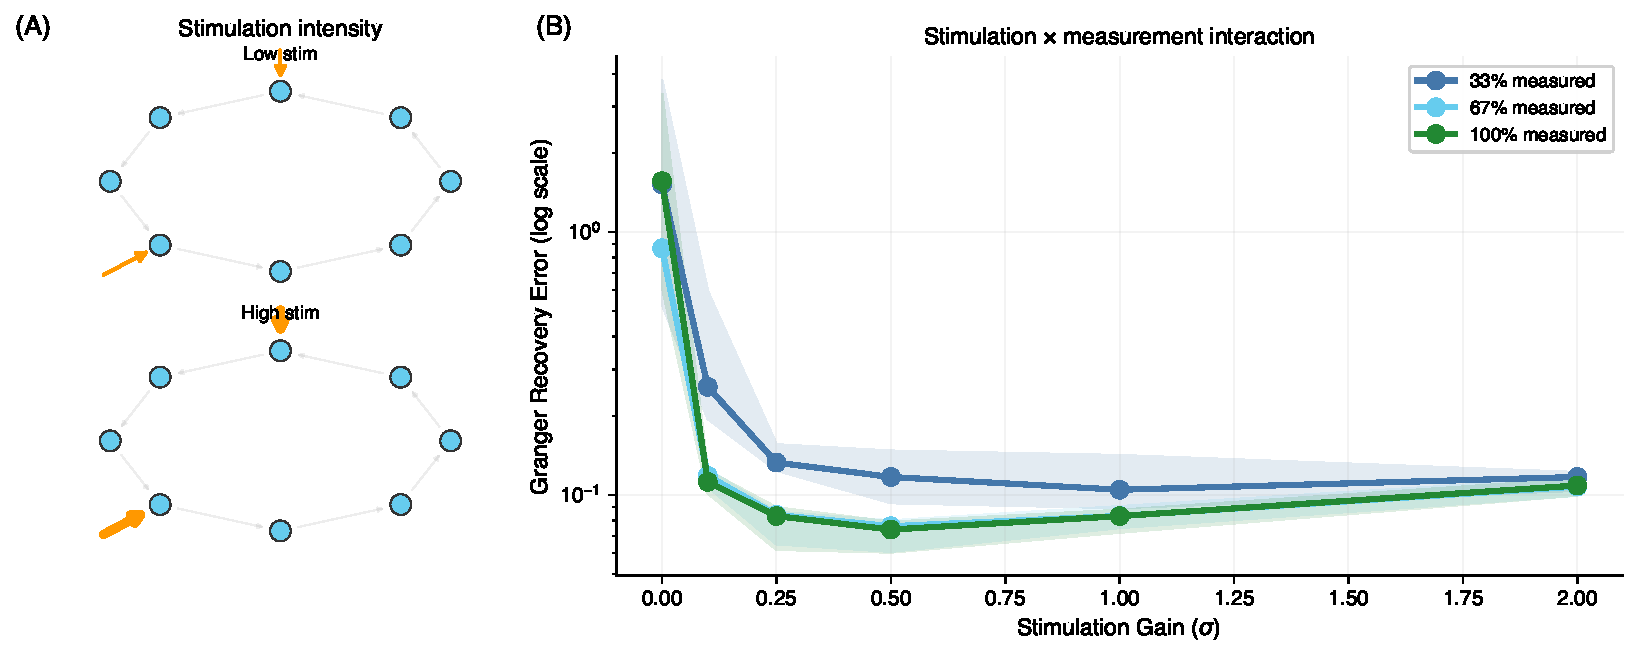
\includegraphics[width=\linewidth]{figures/fig4_stimulation.pdf}
\caption{\textbf{Stimulation-dynamics tradeoff} reveals a critical interaction between stimulation and measurement density ($N=15$, $T=1000$, 10 topologies $\times$ 50 instances). \textbf{(A)} Schematic: extrinsic Gaussian stimulation of varying intensity applied to stimulated nodes. \textbf{(B)} Recovery error vs.\ stimulation gain $\sigma$ for three measurement fractions (33\%, 66\%, 100\%; $5$, $10$, $15$ of $N{=}15$ neurons). At low measurement, the effect is mild. At full measurement, zero stimulation yields substantially degraded recovery because CPG dynamics alone leave $\Sigma_{x,x}$ ill-conditioned, while moderate stimulation ($\sigma \approx 0.5$) yields the best recovery. This confirms the control-estimation tradeoff: stimulation is necessary for identifiability but excessive noise degrades the covariance structure.}
\label{fig:tradeoff}
\end{figure}

\subsection{Measurement Sparsity (E4)}

We isolate the effect of measurement density, holding all other factors at baseline, to quantify how much recovery degrades when only a fraction of neurons can be observed in each session.
We vary the fraction of neurons observed per session from $33\%$ to $100\%$ for $N=15$, $T=1000$.
Full observability ($100\%$) yields error of $0.083$ compared to $0.105$ at $33\%$ measurement (Granger-refined), confirming that measurement sparsity is a significant challenge.
At $33\%$ measurement, the raw estimate ($0.110$) is modestly improved by the Granger-inspired refinement to $0.105$.
The improvement plateaus above $\sim50\%$ measurement fraction (Figure~\ref{fig:sparsity}).

\begin{figure}[ht]
\centering
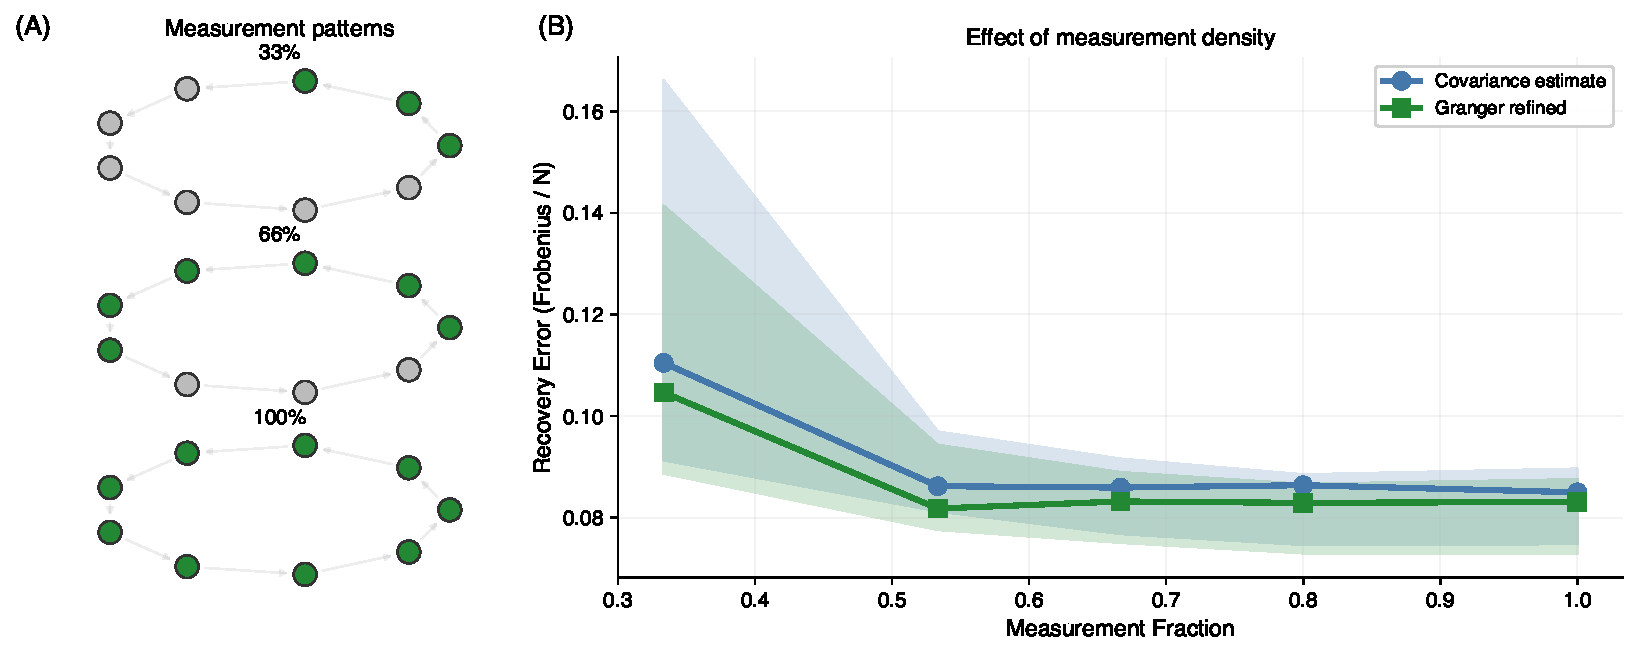
\includegraphics[width=\linewidth]{figures/fig5_sparsity.pdf}
\caption{\textbf{Effect of measurement density on connectivity recovery} for $N=15$, $T=1000$. \textbf{(A)} Schematic: three example measurement patterns at 33\%, 66\%, and 100\% neuron observability (green = measured, gray = unobserved). \textbf{(B)} Median recovery error vs.\ measurement fraction for the raw covariance estimator (blue) and Granger-refined estimator (green), with 95\% bootstrap CI (shaded). Full observability ($100\%$) yields error $0.083$; at $33\%$ the Granger-refined estimate ($0.105$) modestly improves on the raw estimate ($0.110$). 10 topologies $\times$ 50 sessions per condition.}
\label{fig:sparsity}
\end{figure}

\subsection{Nonlinearity Robustness (E5)}

Our estimator assumes $\phi(x) \approx x$ in its core derivation. How badly does this approximation hurt when the true activation is $\tanh$, sigmoid, or ReLU?
We test four nonlinearities at $N=15$ with $66\%$ measurement and $\sigma=1.0$.
$\tanh$ yields the \emph{best} recovery (Granger error $0.083$), while identity and ReLU (for which the linear approximation is exact) perform worse (error $\sim 0.17$).
This occurs because $\tanh$ \emph{bounds} the state values, improving $\kappa(\Sigma_{x,x})$, while unbounded nonlinearities allow state drift, severely degrading the conditioning of $\Sigma_{x,x}$.
Sigmoid achieves intermediate error ($0.132$): its boundedness helps conditioning relative to identity and ReLU, but its non-zero mean ($\phi(0) = 0.5$) biases the covariance estimate.
The Granger-inspired refinement is beneficial across all nonlinearities (Figure~\ref{fig:nonlinearity}).

\begin{figure}[ht]
\centering
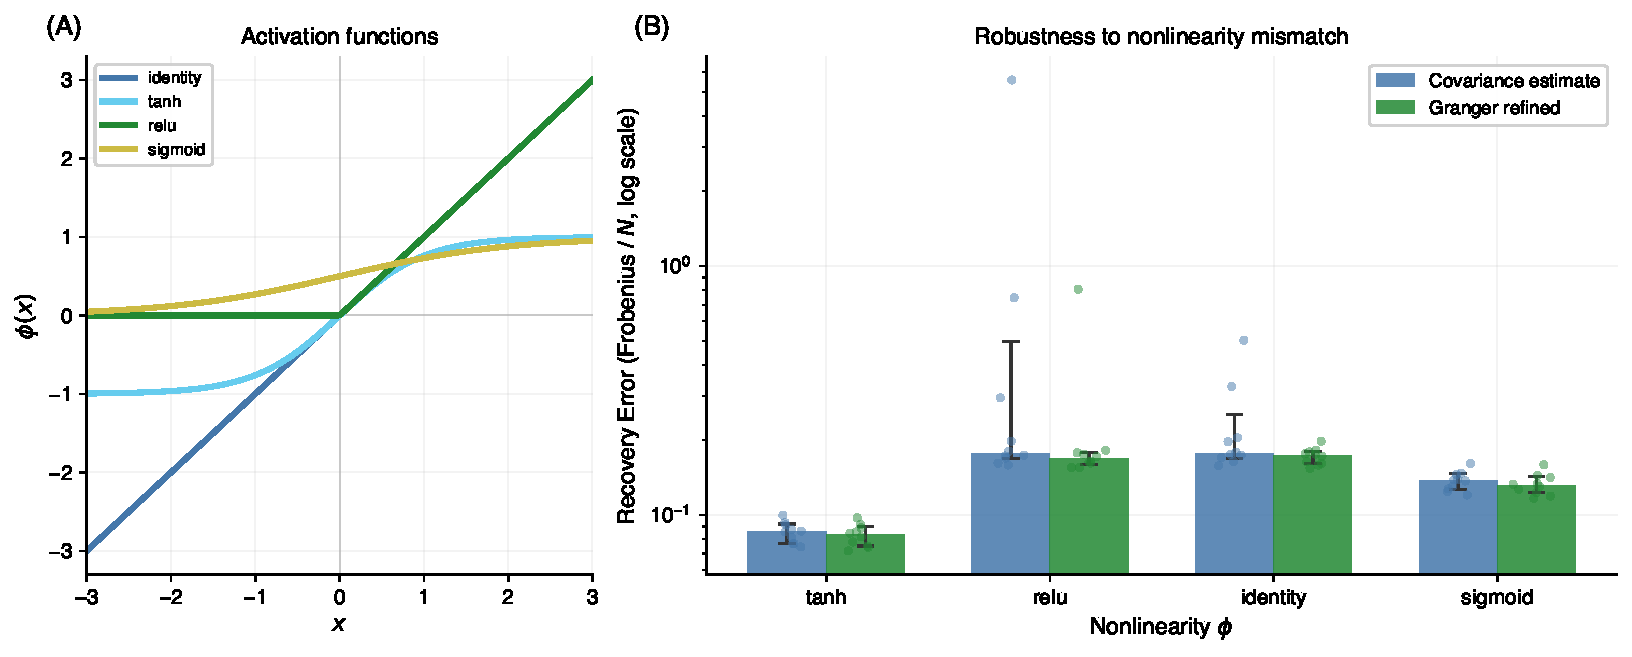
\includegraphics[width=\linewidth]{figures/fig6_nonlinearity.pdf}
\caption{\textbf{Robustness to nonlinearity mismatch} for $N=15$, $T=1000$, $66\%$ measured. \textbf{(A)} The four activation functions tested. \textbf{(B)} Median recovery error (log scale) for the raw estimator (blue) and Granger-refined (green) with bootstrap error bars. Counterintuitively, $\tanh$ yields the \emph{best} recovery ($0.083$) because it bounds state values, improving $\kappa(\Sigma_{x,x})$. Unbounded nonlinearities (identity, ReLU) allow state drift that worsens conditioning. Dots show individual session recoveries (10 topologies $\times$ 50 sessions).}
\label{fig:nonlinearity}
\end{figure}

\subsection{Oracle vs.\ Approximation (E6)}

Theory predicts something counterintuitive: the linear approximation should be \emph{better} than an oracle estimator that knows the true nonlinearity. We test this directly.
A central theoretical prediction of our framework (Section~\ref{sec:app_oracle}) is that the ``incorrect'' linear approximation $\hat{W} = \Sigma_{x_{t+1},x_t}\Sigma_{x_t,x_t}^{-1}$ can outperform the oracle estimator $\hat{W}_{\mathrm{oracle}} = (\Sigma_{x_{t+1},x} - \Sigma_{b,x})\Sigma_{\phi(x),x}^{-1}$ that uses the true nonlinearity $\phi$ and subtracts the input correlation (full derivation in Appendix~\ref{sec:app_oracle}).
We test this by comparing both estimators across stimulation intensities $\sigma \in \{0, 0.1, 0.25, 0.5, 1, 2, 5\}$ for $N=15$, $T=1000$ with $\tanh$ nonlinearity, $66\%$ measurement, and 10 topologies.

The approximation outperforms or matches the oracle at every tested stimulation level (Figure~\ref{fig:oracle}).
Excluding the pathological $\sigma{=}0$ regime where all three estimators fail, the oracle penalty (ratio of oracle error to Granger-refined approximation error) is largest at low stimulation ($\sim2.2\times$ at $\sigma{=}0.1$, $\sim1.7\times$ at $\sigma = 0.25$--$0.5$) and narrows to ${\sim}1.5\times$ for $\sigma \geq 1$.
No crossover point exists: the conditioning penalty from inverting $\Sigma_{\phi(x),x}$ consistently exceeds the bias reduction from using the correct nonlinearity.
This confirms that the linear approximation provides implicit regularization analogous to ridge regression (see Discussion, Section~\ref{sec:discussion}, and Appendix~\ref{sec:app_oracle} for the bias-variance analysis).

\begin{figure}[ht]
\centering
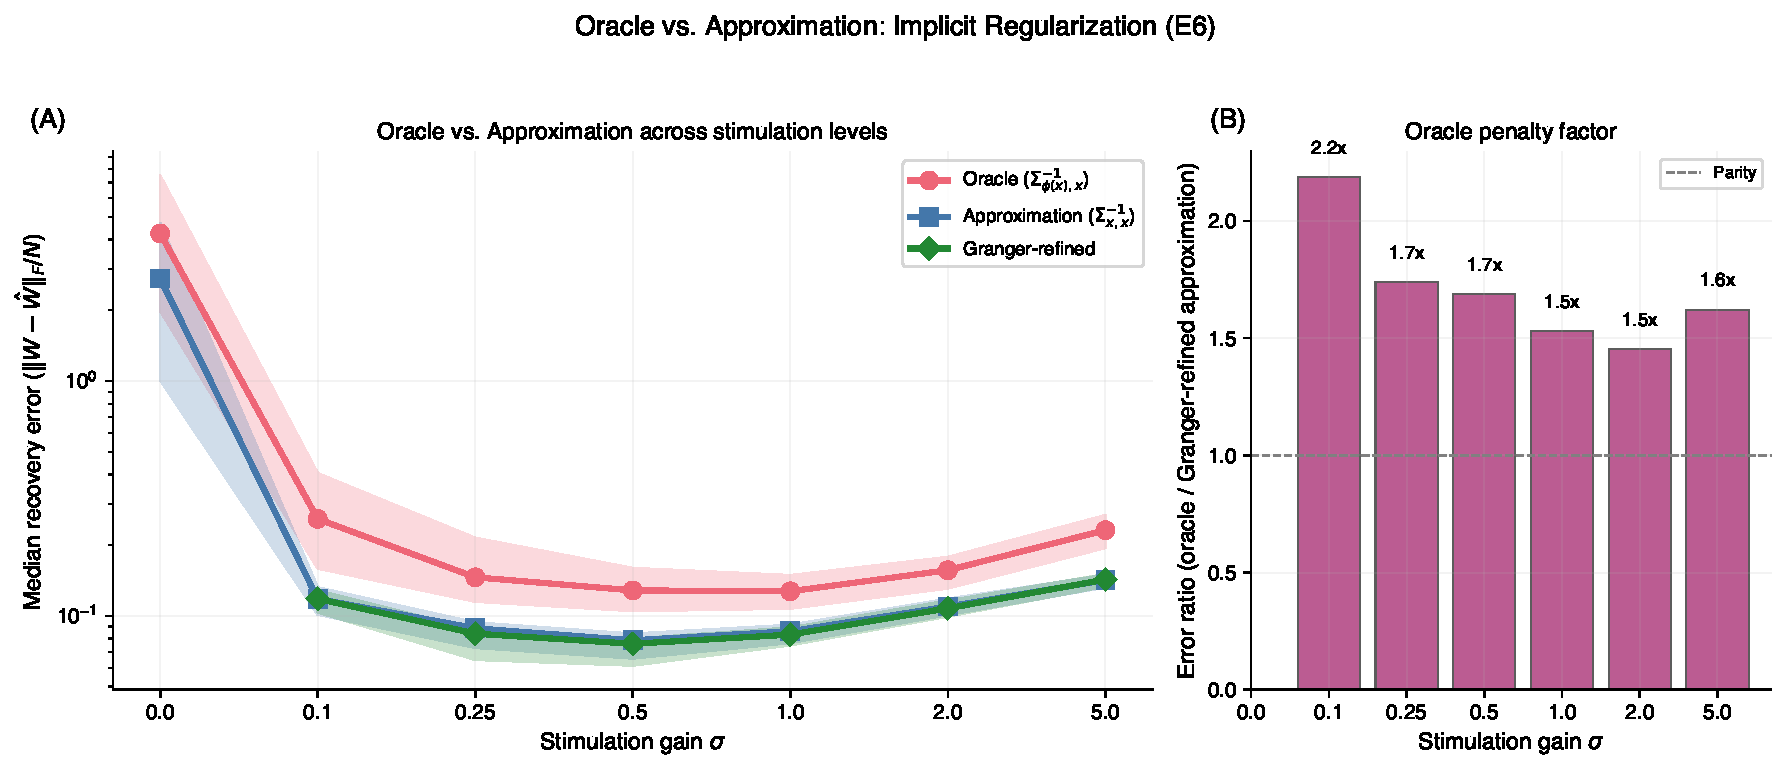
\includegraphics[width=\linewidth]{figures/fig7_oracle_comparison.pdf}
\caption{\textbf{Oracle vs.\ approximation comparison} across stimulation intensities ($N=15$, $T=1000$, $66\%$ measured, $\tanh$, 10 topologies $\times$ 50 instances). \textbf{(A)} Median recovery error (log scale) for the oracle estimator using the true nonlinearity (red), the linear approximation (blue), and the Granger-refined approximation (green). Shaded: 95\% bootstrap CI. The approximation matches or outperforms the oracle at every $\sigma$, with the largest non-pathological gap ($\sim 2.2\times$) at $\sigma{=}0.1$. \textbf{(B)} Oracle penalty factor: ratio of oracle error to Granger-refined approximation error. The oracle never achieves lower error than the Granger-refined approximation, confirming the implicit regularization effect predicted by the bias-variance analysis (Appendix~\ref{sec:app_oracle}).}
\label{fig:oracle}
\end{figure}

\subsection{Stimulation Coverage (E7)}

Experiments E3 and E7 together characterize two orthogonal axes of stimulation design.
E3 (Section~\ref{sec:experiments}) held stimulation \emph{fraction} fixed at $33\%$ and varied stimulation \emph{intensity} (gain $\sigma$).
E7 holds gain fixed at $\sigma=1.0$ and varies the \emph{fraction} of neurons receiving stimulation.

These axes are mechanistically distinct: gain controls the \emph{magnitude} of each neuron's input covariance, while fraction controls the \emph{rank} of the aggregate stimulation covariance $\Sigma_{b^{\mathrm{stim}},b^{\mathrm{stim}}}$.
With $n_{\mathrm{stim}}$ stimulated neurons receiving independent i.i.d.\ noise, the stimulation covariance has rank exactly $n_{\mathrm{stim}}$.
When $n_{\mathrm{stim}} = 0$, the rank is zero: all input directions in state space depend entirely on the CPG, leaving $\Sigma_{x,x}$ ill-conditioned and the estimator unreliable.
Targeting more neurons raises the rank, injecting independent excitation into more directions of state space and improving the conditioning of $\Sigma_{x,x}$.
In practice, stimulation fraction is controlled by the number of neurons expressing a light-sensitive opsin in an optogenetic experiment.

We compare three conditions: no stimulation ($0\%$), moderate coverage ($33\%$, $n_{\mathrm{stim}} = 10$ of $N=30$), and broader coverage ($66\%$, $n_{\mathrm{stim}} = 20$), at fixed $\sigma=1.0$ and $66\%$ measurement.
With zero stimulation, recovery is substantially degraded (error $\approx 0.83$), as the covariance matrix $\Sigma_{x,x}$ has near-zero rank in the stimulation directions.
At $33\%$ coverage, error drops dramatically (to $\approx 0.05$), matching baseline performance.
At $66\%$ coverage, performance is unchanged from $33\%$, confirming that the benefit saturates quickly (Figure~\ref{fig:stim_coverage}).

\begin{figure}[ht]
\centering
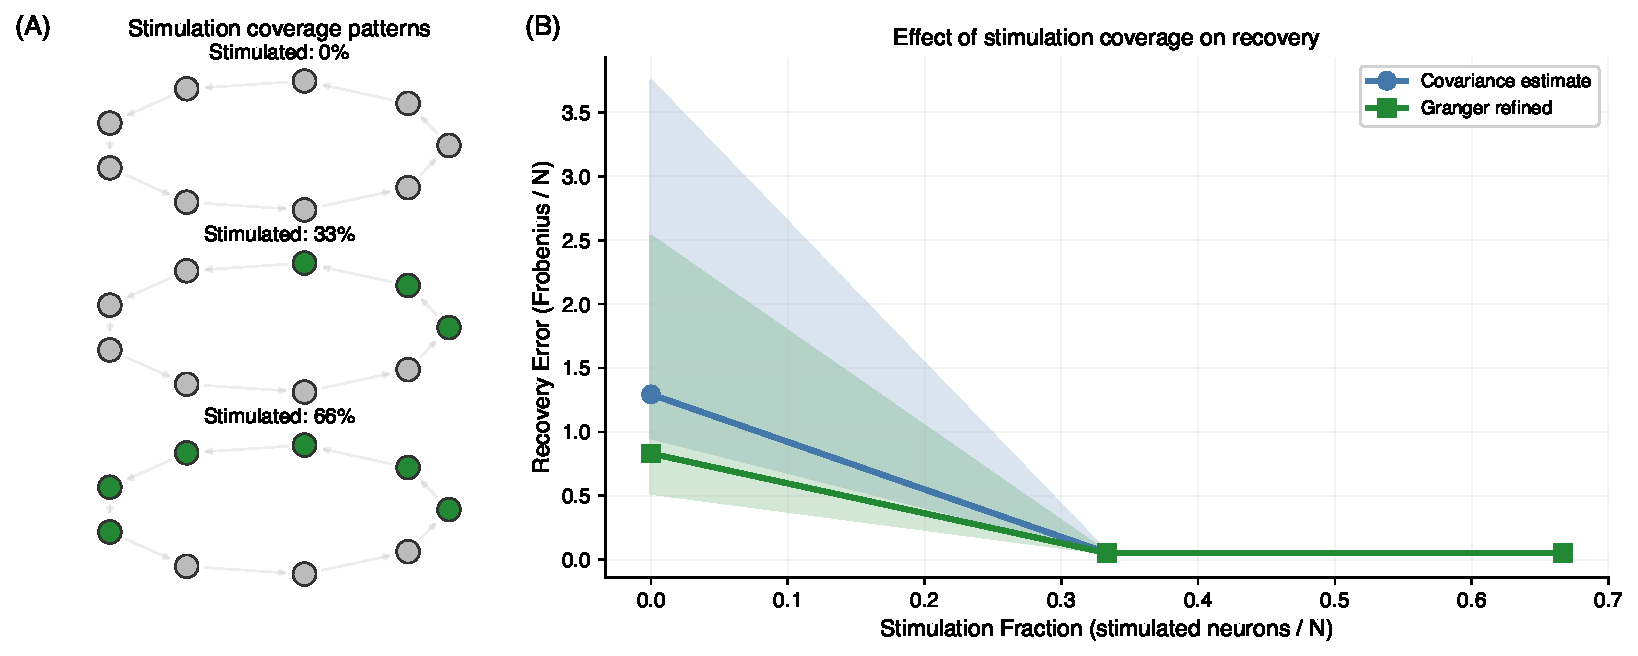
\includegraphics[width=0.7\linewidth]{figures/fig8_stim_fraction.pdf}
\caption{\textbf{Effect of stimulation coverage} on connectivity recovery ($N=30$, $T=1000$, $66\%$ measured, $\sigma=1.0$). \textbf{(A)} Schematic showing three stimulation patterns at $0\%$, $33\%$, and $66\%$ coverage. \textbf{(B)} Recovery error for the covariance estimate (blue) and Granger-refined estimate (green) across the three conditions. Zero stimulation yields substantially degraded recovery (error ${\approx}0.83$) because $\Sigma_{x,x}$ has zero rank in the stimulation directions; $33\%$ coverage drops error to ${\approx}0.05$, matching baseline performance; $66\%$ shows no further improvement, confirming rapid saturation. Shaded: 95\% bootstrap CI. Stimulation fraction controls the \emph{rank} of the input covariance, independently of stimulation intensity (E3).}
\label{fig:stim_coverage}
\end{figure}

% ============================================================================
\section{Related Work}
\label{sec:related}
% ============================================================================

Our approach combines ideas from several distinct literatures: neural connectivity inference, Granger causality analysis, compressed sensing, matrix completion, and system identification. We briefly situate the method relative to each.

\paragraph{Neural connectivity inference.}
Inferring functional connectivity from neural recordings is a longstanding challenge.
Modern calcium imaging enables simultaneous recording of hundreds of neurons in neural circuits \citep{kato2015global, yemini2021neuropal}, but full coverage in a single session remains difficult.
Generalized linear models (GLMs) \citep{pillow2008spatio} provide a principled regression-based framework for inferring directed connectivity, though they assume all relevant neurons are observed.
\citet{linderman2014discovering} extend this line by jointly inferring a latent weighted graph and Hawkes-process dynamics under a fully Bayesian random-graph prior; in contrast, our method is non-parametric in the dynamics, recovers $W$ from second moments alone, and assumes only that the noise driving the recurrent network is approximately uncorrelated with the state.
Transfer entropy \citep{schreiber2000measuring} offers a model-free alternative that captures nonlinear interactions, but is sensitive to unobserved confounders.
More broadly, \citet{janzing2010causal} show that even under partial observability, causal structure is identifiable when the joint distribution admits an algorithmically simple factorization aligned with the true graph; our pooling-then-inverting strategy can be read as a second-order, finite-sample analog of this principle, exploiting that distinct session masks expose complementary marginals of a single underlying causal mechanism.
\citet{soudry2015shotgun} introduced the ``shotgun'' multi-session sampling design, in which a small, randomly varying subset of neurons is observed at each epoch, and showed that an EM-based generalized linear model can disentangle direct from latent-mediated effects under this scheme; our estimator targets the same observation model but pools second-order covariance statistics across sessions and inverts globally in closed form, trading the GLM likelihood for a simpler convex moment-matching step.
Our covariance-based approach is complementary: it explicitly handles partial observations by accumulating statistics across sessions.

\paragraph{Granger causality in neuroscience.}
Granger causality \citep{granger1969investigating} quantifies whether the past of one time series improves prediction of another.
\citet{seth2015granger} review its application to neural data, noting challenges with nonlinear dynamics and confounding latent variables.
Our Granger-inspired refinement uses a simpler criterion, comparing contemporaneous and lagged covariances, rather than full autoregressive modeling.

\paragraph{Compressed sensing and sparse recovery.}
Compressed sensing methods have been applied to reconstruct synaptic connections from subsampled neural recordings \citep{candes2006robust}.
\citet{brunton2016discovering} applied sparse identification to discover governing equations of dynamical systems.
Our approach differs in that we recover a full matrix rather than a sparse vector, and leverage temporal covariance structure rather than random projections.

\paragraph{Matrix completion.}
Matrix completion (recovering a matrix from a subset of its entries) has been studied extensively under low-rank assumptions \citep{candes2009exact}.
Nuclear norm minimization can recover a rank-$r$ matrix of size $N \times N$ from $O(rN \log^2 N)$ uniformly sampled entries.
Our problem shares the high-level structure (recover a matrix from partial information) but differs in two key respects: the connectivity matrix $W$ is sparse rather than low-rank, and the ``observations'' are not direct entries of $W$ but temporal covariance statistics accumulated across recording sessions.
Nevertheless, the coupon-collector argument for session coverage (Section~\ref{sec:discussion}) mirrors the sampling requirements in matrix completion theory, and both frameworks share the insight that structured matrices can be recovered from far fewer measurements than their ambient dimension would suggest.

\paragraph{Systems identification.}
Classical system identification \citep{ljung1998system} addresses parameter estimation in dynamical systems, including vector autoregressive (VAR) models for multivariate time series.
Our estimator can be viewed as a single-lag VAR model applied to partially observed data, with the key difference that we accumulate covariance statistics across sessions with different observation masks.
Reservoir computing \citep{sussillo2009generating} has shown that random recurrent networks can generate complex temporal patterns, motivating our use of chaotic reservoir CPGs.
Our method is distinct from all of the above in that it operates with partial observations \emph{by design}, accumulating sufficient statistics across sessions with different measurement masks before a single global inversion---a property none of the cited methods share.

% ============================================================================
\section{Discussion}
\label{sec:discussion}
% ============================================================================

\paragraph{The covariance estimator works but has limitations.}
Our results demonstrate that the covariance-based estimator $\hat{W} = \Sigma_{x_{t+1},x_t}\Sigma_{x_t,x_t}^{-1}$ can recover connectivity from partial measurements, consistently outperforming chance baselines for small networks.
For larger networks, the estimator's performance degrades due to ill-conditioning: when only $\sim33\%$ of neurons are observed per session, the empirical covariance matrix may be rank-deficient, leading to high-variance estimates.
This suggests that increasing the measurement fraction or the number of recording sessions is critical for scaling to larger circuits.

\paragraph{Error decomposition: CPG correlation dominates.}
Before dissecting individual pipeline components, it helps to understand \emph{why} the estimator works and where its residual error comes from.
The independence assumption $\text{Cov}(b_t, x_t) \approx 0$ is only partially justified: the extrinsic stimulation is truly independent ($\text{Cov}(\text{stim}_t, x_t) = 0$ by construction), but the CPG drive depends on the current state through $\text{cpg}(x_t)$, so $\text{Cov}(\text{cpg}_t, x_t) \neq 0$.
Quantitatively, $\|e_2\|_F$ (input correlation) is ${\sim}3\times$ larger than $\|e_1\|_F$ (model mismatch), making the unmodeled state-dependent drive the \emph{dominant} error source, not the linear approximation (Figure~\ref{fig:dynamics}D).
CPG nodes can be partially identified from data: they exhibit higher activity variance than non-CPG nodes, enabling detection via a simple variance threshold (F1 score $\sim 0.8$).
This suggests a natural extension: downweighting detected CPG nodes during covariance accumulation could mitigate the dominant error source, a direction we leave to future work.

\begin{figure}[!tbp]
\centering
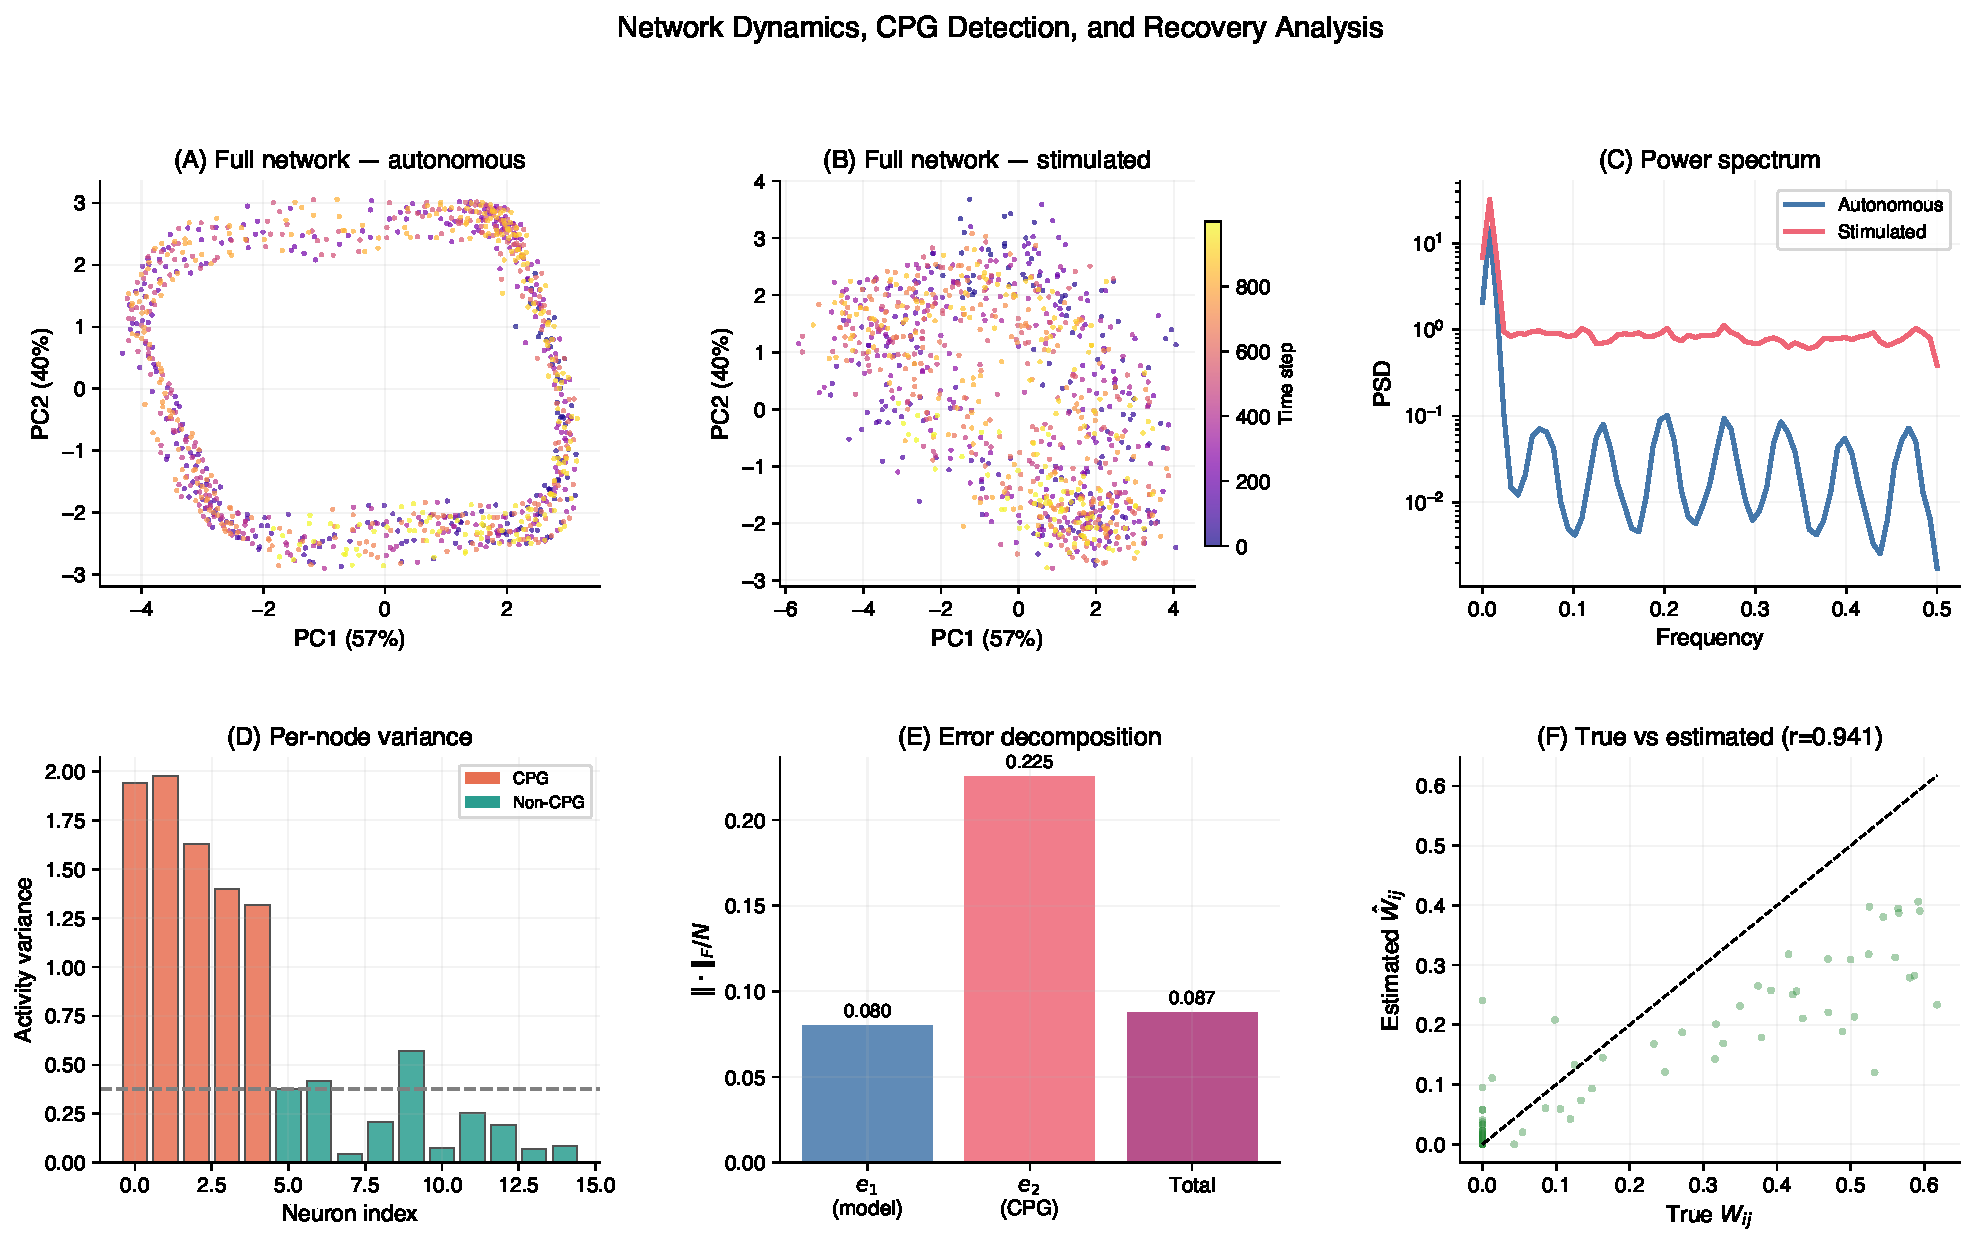
\includegraphics[width=\linewidth]{figures/fig9_dynamics.pdf}
\caption{\textbf{Network dynamics, error decomposition, and recovery quality} ($N{=}15$, $\phi{=}\tanh$, $\rho(W){=}1.0$).
\textbf{(A--B)} PCA phase portraits of network activity ($X \in \mathbb{R}^{T \times N}$ projected onto PC1--PC2, colored by time via plasma colormap: dark purple $\to$ yellow). (A) Under autonomous dynamics ($\sigma=0$), the trajectory is confined to a low-dimensional manifold shaped by intrinsic oscillators. (B) Under stimulation ($\sigma=1.0$), the trajectory fills a larger volume in PC space, reflecting the expanded covariance coverage that enables estimation.
\textbf{(C)} Power spectral density (Welch's method) averaged across neurons. Autonomous dynamics (blue) show concentrated spectral peaks at intrinsic-oscillator frequencies; stimulated dynamics (red) exhibit a flatter spectrum reflecting white-noise input.
\textbf{(D)} Error decomposition: $\|e_1\|_F/N$ (model mismatch) vs.\ $\|e_2\|_F/N$ (unmodeled-drive correlation with state) vs.\ total estimation error $\|\hat{W} - W\|_F/N$. $e_1$ and $e_2$ are Frobenius norms of the individual error components (Eq.~\ref{eq:error}); the total can be smaller because these components partially cancel across matrix entries. For this representative topology, $e_2$ is ${\sim}2.8\times$ larger than $e_1$ (median across topologies: ${\sim}3\times$), identifying the unmodeled state-dependent drive (here, CPG input) as the dominant error source.
\textbf{(E)} Scatter plot of true off-diagonal weights $W_{ij}$ (horizontal) vs.\ Granger-refined estimates $\hat{W}_{ij}$ (vertical) for this representative topology. Pearson $r = 0.94$; dashed line: $y=x$. Median raw-estimator correlation across all 10 topologies: $r = 0.90$.}
\label{fig:dynamics}
\end{figure}

\paragraph{Granger-inspired refinement is consistently beneficial.}
The structural priors (no autapses, non-negativity) account for the bulk of improvement over the unprocessed estimate, with the no-autapse constraint being most impactful (Section~\ref{sec:methods}).
The Granger-inspired refinement adds the lagged-covariance sparsity pattern (Appendix~\ref{sec:app_granger_rule}), improving precision from $0.30$ to $0.40$ while maintaining recall at $0.96$ (E2, Figure~\ref{fig:granger}).
For practical circuit mapping, a precision of $0.40$ means roughly $60\%$ of predicted edges are spurious---sufficient as a screening tool that narrows the candidate edge set for targeted validation, but not for definitive wiring inference without additional evidence.

\paragraph{The linear approximation provides implicit regularization.}
A surprising finding is that the approximate estimator (using $\Sigma_{x,x}$) outperforms the natural plug-in oracle estimator that inverts $\Sigma_{\phi(x),x}$ with known $\phi$ and $b$ (Appendix~\ref{sec:app_oracle} discusses how a hypothetical ``split'' oracle with separately estimated $D$ would close part of this gap).
The Stein--Price identity (Appendix~\ref{sec:app_price}) explains why: $\Sigma_{\phi(x),x} = D \Sigma_{x,x}$ where $D = \mathrm{diag}(\mathbb{E}[\mathrm{sech}^2(x_i)])$ with $0 < d_i < 1$.
Because $\tanh$ compresses large values, the oracle covariance is a \emph{row-compressed} version of $\Sigma_{x,x}$, making its condition number potentially worse: $\kappa(\Sigma_{\phi(x),x}) \leq \kappa(\Sigma_{x,x}) \cdot d_{\max}/d_{\min}$.
When state variances are heterogeneous across neurons, this ratio can be large, amplifying noise in the oracle inversion.
The ``incorrect'' linear approximation using $\Sigma_{x,x}$ is better-conditioned, acting as implicit regularization, analogous to how ridge regression (biased) can outperform OLS (unbiased but high-variance), or how James--Stein shrinkage reduces total risk by trading bias for variance.
The E6 experiment (Section~\ref{sec:experiments}, Figure~\ref{fig:oracle}) confirms this prediction empirically: the approximation matches or outperforms the oracle at all seven stimulation intensities tested, with the largest non-pathological gap ($\sim2.2\times$ in the Granger-refined approximation) at $\sigma = 0.1$.

\paragraph{Stimulation coverage: a practical experimental knob.}
Our experiments reveal two complementary axes of stimulation design: \emph{intensity} (E3) and \emph{coverage} (E7).
Stimulation gain controls the \emph{magnitude} of the input covariance, while stimulation fraction controls its \emph{rank}, the number of independent input directions exciting the network.
The E7 results show that zero stimulation yields substantially degraded recovery because CPG-driven dynamics alone leave $\Sigma_{x,x}$ ill-conditioned.
At $33\%$ stimulation ($10$ of $N=30$ neurons), error drops substantially, and performance plateaus beyond $\sim 33\%$ stimulation coverage.
This has a direct practical implication: in optogenetic experiments, an experimenter need not achieve pan-neuronal actuator expression. Targeting roughly one-third of neurons suffices, provided stimulation intensity is moderate ($\sigma \approx 0.5$--$1.0$).
Combined with the E3 finding that excessive stimulation degrades recovery, this defines a practical operating regime: moderate gain applied to a modest subset of neurons.

\paragraph{Connection to neuroscience experiments.}
In practice, the ``sessions'' in our framework correspond to separate recording sessions of the same animal or circuit, where different neurons are visible due to imaging field of view, indicator expression, or optical access.
The key requirement is that sessions share the same underlying connectivity $W$, a reasonable assumption for short-term experiments in small circuits where the connectome is conserved.
Tools for consistent neuron identification across sessions, such as NeuroPAL \citep{yemini2021neuropal}, make this framework directly applicable to real experimental data.

\paragraph{Identifiability conditions.}
$W$ is uniquely recoverable if and only if every neuron pair $(i,j)$ is co-observed in at least one session ($n_{ij} \geq 1$ for all $i,j$) and $\Sigma_{x,x}$ is invertible.
Necessity follows because unobserved pairs leave covariance entries unconstrained; sufficiency follows from $W = \Sigma_1 \Sigma_0^{-1}$.
For random measurement patterns where each neuron is observed independently with probability $p$, a union bound over $N^2$ pairs gives:
\begin{equation}
    K \geq \frac{\log(N^2/\delta)}{p^2} \quad \Rightarrow \quad \Pr(\text{all pairs covered}) \geq 1 - \delta
\end{equation}
This is tight up to constants, matching a coupon-collector argument where each session yields $\sim (pN)^2$ pair-coupons.
Beyond this \emph{structural} identifiability, \emph{practical} identifiability demands that $\Sigma_{x,x}$ is well-conditioned for stable inversion.
Our experiments (Section~\ref{sec:experiments}) show that measurement density directly controls $\kappa(\Sigma_{x,x})$, creating a gap between the two.

\paragraph{Robustness to measurement noise.}
When observation noise is present, Eq.~\eqref{eq:estimator} shows that the estimator becomes ridge-regularized: $\hat{W} = W\Sigma_{x,x}(\Sigma_{x,x} + \sigma_\epsilon^2 I)^{-1}$, which shrinks estimates toward zero.
In systematic tests (E8, 10 topologies, baseline configuration), at $\sigma_\epsilon = 0.1$ (relative to state std $\sim 0.8$) the Granger-refined error increases by $\sim 2\%$, and at $\sigma_\epsilon = 0.5$ by $\sim 32\%$.
The graceful degradation follows from the ridge structure: noise regularizes the inversion rather than corrupting it catastrophically.

\paragraph{Limitations.}
(1)~The Stein--Price bound assumes Gaussian states, but our states are driven by a chaotic reservoir through $\tanh$; the bound is directionally correct but not formally tight for non-Gaussian distributions.
(2)~Our experiments use excitatory networks ($W_{ij} \geq 0$), where the Perron--Frobenius theorem \citep{horn1985matrix} guarantees a unique real dominant eigenvalue and simplifies spectral radius control.
Real circuits include inhibitory connections (mixed-sign $W$); extending the method requires relaxing the non-negativity modeling prior.
Preliminary tests with mixed-sign weights yield qualitatively similar recovery accuracy for the covariance estimator itself, since the estimator $\hat{W} = \Sigma_{y_{t+1},y_t}\Sigma_{y_t,y_t}^{-1}$ does not assume sign constraints.
(3)~We compare against per-session VAR (OLS) and Ridge-GLM ($\ell_2$, $\alpha{=}1$) baselines (E2). Both underperform our accumulate-then-invert estimator ($58\%$ and $36\%$ worse, respectively), confirming that global covariance pooling is the critical design choice. Comparison against full-data GLMs with Poisson link \citep{pillow2008spatio} (appropriate for spike data rather than our continuous activity) is a direction for future work.
(4)~Our experiments span $N \in \{15, 159, 300\}$, motivated by biologically relevant circuit scales: from the lobster stomatogastric ganglion (${\sim}30$ neurons; \citep{marder2007understanding}) to \textit{C.~elegans} (302 neurons; \citep{white1986structure}). The method itself places no upper bound on $N$; the computational bottleneck is the $O(N^3)$ covariance inversion, for which efficient iterative and sparse solvers exist, and recent advances in AI-discovered linear-algebra algorithms \citep{fawzi2022discovering} suggest this ceiling is not fundamental.
(5)~Our primary results assume noiseless observations; noise robustness tests (E8) show graceful degradation ($2\%$ at $\sigma_\epsilon = 0.1$, $32\%$ at $\sigma_\epsilon = 0.5$).
(6)~We assume a fixed weight matrix $W$ shared across recording sessions, which holds on the short timescales typical of optogenetic experiments; biological synapses are plastic on longer timescales, so the recovered $\hat{W}$ should be interpreted as a snapshot of effective connectivity rather than a permanent wiring diagram.

% ============================================================================
\section{Conclusion}
\label{sec:conclusion}
% ============================================================================

We have studied a partial-window system identification problem in which a recurrent network is observed only through varying subsets of its state variables across sessions, and asked whether the connectivity matrix $W$ is nevertheless recoverable.
The answer is yes when (i) every pair of neurons is co-observed at least once, (ii) the underlying weights do not drift between sessions, and (iii) covariances are pooled \emph{before} a single global pseudoinverse rather than fit per session.
Three findings refine that answer into something more useful for designers of such estimators.

First, dropping the network's nonlinearity from the estimator can \emph{improve} recovery: the natural plug-in oracle that uses the true nonlinearity inverts a row-compressed covariance whose worse conditioning outweighs its lower bias---an instance of James--Stein-style implicit regularization (E6). Practically, this removes the need to characterize the neuronal transfer function before estimating $W$.
Second, partial observability creates a control--estimation tradeoff: stimulation excites otherwise-unobservable network modes (good for identifiability) but disrupts intrinsic dynamics (bad for studying them), with the optimum interior to the design space (E3, E7).
Third, an error decomposition (Eq.~\ref{eq:error}) cleanly separates two failure modes---approximating a nonlinear circuit as linear ($e_1$) and unmodeled state-dependent drive ($e_2$)---and shows the second to be ${\sim}3\times$ larger in our setting. The estimator's remaining error is therefore not principally a math-approximation problem but a problem of unmodeled autonomous dynamics, which points to the next concrete direction: jointly estimating $W$ alongside a model of the intrinsic drive.

Several directions merit future investigation.
Extending the framework to real neural recordings, particularly \textit{C.~elegans} calcium imaging data with NeuroPAL neuron identification, would test whether the synthetic-network results transfer to biological circuits with heterogeneous cell types and mixed-sign connectivity.
Structured stimulation protocols (e.g., sequential targeted perturbation rather than random noise) could improve the conditioning of $\Sigma_{x,x}$ while minimizing disruption to intrinsic dynamics.
Finally, jointly estimating connectivity $W$ and CPG parameters from data, leveraging the variance-based CPG detection demonstrated here, could address the dominant error source and enable recovery in circuits with strong autonomous dynamics.

% ============================================================================
% References
% ============================================================================

% ============================================================================
\paragraph{Code and data availability.}
All code, experiment configurations, and per-rep result JSONs are available at \url{https://github.com/qsimeon/sparse_matrix_recovery}.

\bibliographystyle{plainnat}
\bibliography{references}

% ============================================================================
\newpage
\appendix
\section{Supplementary Material}
\label{sec:appendix}
% ============================================================================

\subsection{Derivation Details: Stein--Price Identity for Model Mismatch}
\label{sec:app_price}

For jointly Gaussian $x \sim \mathcal{N}(0, \Sigma)$ and differentiable $f$, the Stein--Price identity states:
\begin{equation}
    \mathbb{E}[f(x_i) x_j] = \Sigma_{ij} \, \mathbb{E}[f'(x_i)]
\end{equation}
Applying this with $f = \tanh$ (so $f' = \text{sech}^2$):
\begin{equation}
    \mathbb{E}[\tanh(x_i) x_j] = \Sigma_{ij} \, \mathbb{E}[\text{sech}^2(x_i)]
\end{equation}
Therefore $\Sigma_{\phi(x),x} = D \Sigma_{x,x}$ where $D = \text{diag}(\mathbb{E}[\text{sech}^2(X_i)])$ with $X_i \sim \mathcal{N}(0, \sigma_i^2)$.
The model mismatch in $e_1$ reduces to $W(D - I)$, with $\|e_1\|_F \leq \|W\|_F \max_i(1 - D_{ii})$.
For small state variance, $1 - \mathbb{E}[\text{sech}^2(X_i)] \approx \sigma_i^2 - 2\sigma_i^4 + O(\sigma_i^6)$, giving the $O(\sigma^2)$ bound used in Section~\ref{sec:methods}.
For large variance, $\mathbb{E}[\text{sech}^2(X_i)] \to 0$ as $\sigma_i \to \infty$, so the mismatch approaches $W \cdot (-I) = -W$.
Note that $\mathbb{E}[x_i^3 x_j] = 3\sigma_i^2 \Sigma_{ij} \neq 0$ for Gaussians (degree-4 moment), correcting a common misconception that this vanishes by symmetry.

\subsection{Identifiability Proof Sketch}
\label{sec:app_ident}

\textbf{Theorem.} Under the linear model $x_{t+1} = Wx_t + \varepsilon_t$ with invertible $\Sigma_0 = \mathbb{E}[x_t x_t^T]$, the weight matrix $W$ is uniquely recoverable from measurement pattern $\{\mathcal{M}_k\}_{k=1}^K$ if and only if $n_{ij} \geq 1$ for all $i,j$, where $n_{ij} = |\{k : i \in \mathcal{M}_k \wedge j \in \mathcal{M}_k\}|$.

\emph{Sufficiency}: If $n_{ij} \geq 1$ for all pairs, every entry of $\Sigma_0$ and $\Sigma_1 = \mathbb{E}[x_t x_{t-1}^T]$ is estimable from co-observed samples. Since $W = \Sigma_1 \Sigma_0^{-1}$, $W$ is uniquely determined.

\emph{Necessity}: If $n_{ij} = 0$ for some pair, the entries $(\Sigma_0)_{ij}$ and $(\Sigma_1)_{ij}$ are never directly observed. Different completions of the covariance matrices can yield different $W$, so $W$ is not structurally identifiable.

For random measurement with per-neuron observation probability $p$, a union bound gives $K \geq \log(N^2/\delta) / p^2$ sessions suffice for all-pairs coverage with probability $\geq 1-\delta$.

\textbf{Scope.} This identifiability statement is for the linearized estimand: it characterizes when the matrix $W$ that minimizes $\|x_{t+1} - W x_t\|^2$ in expectation is unique. Under the paper's actual nonlinear dynamics $x_{t+1} = W\phi(x_t) + b_t$, the same coverage condition is necessary for our covariance-pooling estimator to recover the linear estimand $W \Sigma_{\phi(x),x_t} \Sigma_{x_t,x_t}^{-1}$ uniquely; recovery of the underlying nonlinear generator $W$ additionally relies on the bias bound of \S\ref{sec:methods} and the empirical James--Stein effect of \S\ref{sec:experiments}.

\subsection{Why the Oracle Can Be Worse: Bias-Variance Analysis}
\label{sec:app_oracle}

The oracle estimator $\hat{W}_{\text{oracle}} = (\hat{\Sigma}_{x_{t+1},x} - \hat{\Sigma}_{b,x}) \hat{\Sigma}_{\phi(x),x}^{-1}$ uses the true nonlinearity $\phi$ and input statistics, where hats denote finite-sample estimates.
With infinite data, the oracle recovers $W$ exactly; in practice, the finite-sample estimation error $E_{\text{samp}} = \hat{\Sigma}_{x_{t+1},x} - \Sigma_{x_{t+1},x}$ is amplified by the covariance inversion, and more so when the inverted matrix is ill-conditioned.
By the Stein--Price identity, $\Sigma_{\phi(x),x} = D \Sigma_{x,x}$ where $D = \text{diag}(\mathbb{E}[\text{sech}^2(x_i)])$ with $0 < d_i < 1$.
This makes $\Sigma_{\phi(x),x}$ a \emph{row-compressed} version of $\Sigma_{x,x}$, with potentially worse conditioning: $\kappa(\Sigma_{\phi(x),x}) \leq \kappa(\Sigma_{x,x}) \cdot d_{\max}/d_{\min}$.
Defining $\Delta = D - I$ (the linearization error; each diagonal entry satisfies $-1 < \Delta_{ii} < 0$), the approximation outperforms the oracle when its bias is smaller than the oracle's excess variance:
\begin{equation}
    \underbrace{\|W\|_F \|\Delta\|_2 + \|\Sigma_{b,x}\|_F \|\Sigma_{x,x}^{-1}\|_2}_{\text{approximation bias}} < \underbrace{\|E_{\text{samp}}\|_F \big(\|\Sigma_{\phi(x),x}^{-1}\|_2 - \|\Sigma_{x,x}^{-1}\|_2\big)}_{\text{oracle excess variance}}
\end{equation}
The left side bounds the approximation's total error via submultiplicativity: model mismatch $\|W\Delta\|_F$ plus input correlation $\|\Sigma_{b,x}\Sigma_{x,x}^{-1}\|_F$ (which the oracle removes by subtracting $\hat{\Sigma}_{b,x}$).
The right side captures how the same finite-sample noise $E_{\text{samp}}$ is amplified \emph{more} through the oracle's worse-conditioned $\Sigma_{\phi(x),x}^{-1}$ than through the approximation's $\Sigma_{x,x}^{-1}$.
When state variances are heterogeneous across neurons (common in biological networks), $d_{\max}/d_{\min}$ can be large, making the oracle unstable.
This conditioning penalty is a property of the natural plug-in oracle that estimates $\hat\Sigma_{\phi(x),x}$ as a single sample cross-covariance: a hypothetical ``split'' oracle that estimated $\hat D$ separately and inverted $\hat\Sigma_{x,x}$ would coincide with our oracle in the population limit (both equal $W$ for $b{=}0$ by associativity) but would inherit the better conditioning of $\Sigma_{x,x}^{-1}$, reducing the gap to the linear approximation. The E6 effect therefore reflects two compounding factors---oracle design and implicit James--Stein-style shrinkage---and Figure~\ref{fig:oracle} should be read as a comparison against the natural plug-in oracle, not the optimal one.
This is a concrete instance of the bias-variance tradeoff: like ridge regression or James--Stein shrinkage, a biased estimator with lower variance can achieve better total risk.

\subsection{Granger-Inspired Non-Causality Rule: Derivation and Scope}
\label{sec:app_granger_rule}

Section~\ref{sec:granger} introduced the sparsity rule $W_{ij} := 0$ wherever $\hat{\Sigma}_{x_t,x_t}(i,j) > \hat{\Sigma}_{x_{t+1},x_t}(i,j)$.
Here we derive it from the dynamics model and state its scope precisely.

\paragraph{Population-level justification.}
Under $x_{t+1} = W\phi(x_t) + b_t$ with Gaussian state $x_t \sim \mathcal{N}(0,\Sigma)$ and the Stein--Price identity, the lag-1 cross-covariance decomposes as
\begin{equation}
    \Sigma_{x_{t+1},x_t}(i,j) \;=\; \sum_{k} W_{ik} \, D_k \, \Sigma_{kj} \;+\; \mathrm{Cov}(b_{i,t}, x_{j,t}),
    \label{eq:lag1_expansion}
\end{equation}
where $D_k = \mathbb{E}[\mathrm{sech}^2(x_k)] \in (0,1)$.
The direct contribution of edge $j \to i$ is $W_{ij} D_j \Sigma_{jj}$, which is \emph{positive} whenever $W_{ij} > 0$ (since $D_j > 0$ and $\Sigma_{jj} > 0$).
If, in the population limit, $\Sigma_{ij} > \Sigma_{x_{t+1},x_t}(i,j)$, then the correlation from $j$ at time $t$ to $i$ at time $t{+}1$ is \emph{weaker} than the contemporaneous correlation---contradicting the existence of a positive direct $j \to i$ edge.
Hence $W_{ij} > 0 \;\Rightarrow\; \Sigma_{ij} \leq \Sigma_{x_{t+1},x_t}(i,j)$, and by contraposition:
\[
    \Sigma_{ij} > \Sigma_{x_{t+1},x_t}(i,j) \;\Rightarrow\; W_{ij} = 0.
\]

\paragraph{Relationship to classical Granger causality.}
Classical Granger causality~\citep{granger1969investigating} tests whether including lagged $x_j$ reduces the one-step prediction error for $x_i$ beyond using $x_i$'s own past.
In a correctly specified VAR(1) with infinite data, this reduces to asking whether $W_{ij} \neq 0$, typically answered with an F-test on nested residual variances.
Our rule preserves the same intuition---\emph{future informativeness beyond present informativeness}---but replaces the residual-variance test with a direct inequality on pooled lag-0 and lag-1 covariance entries.
This is cheaper, avoids distributional assumptions about the residuals, and scales naturally to the $K=50$ partially-observed session regime, but it forfeits the statistical interpretability of a p-value.
We therefore call the refinement \emph{Granger-inspired} rather than Granger causality.

\paragraph{Scope and caveats.}
The derivation establishes three strict limits on when the rule is safe:
\begin{enumerate}
    \item \textbf{Non-negativity prior.} The argument ``$W_{ij} > 0 \Rightarrow$ positive direct contribution to $\Sigma_{x_{t+1},x_t}(i,j)$'' requires $W_{ij} \geq 0$. With mixed-sign weights, a negative edge could reduce the lag-1 covariance relative to the lag-0 and satisfy the inequality falsely, producing a spurious zero. The rule is only safe under the excitatory-network prior (Section~\ref{sec:formulation}).
    \item \textbf{Off-path sign-cancellation.} Eq.~\eqref{eq:lag1_expansion} sums contributions from all length-1 paths plus $\mathrm{Cov}(b_{i,t},x_{j,t})$. The contraposition $\Sigma_{ij}>\Sigma_{x_{t+1},x_t}(i,j)\Rightarrow W_{ij}{=}0$ requires both the direct term $W_{ij}D_j\Sigma_{jj}$ and the off-path sum $\sum_{k\neq j}W_{ik}D_k\Sigma_{kj}+\mathrm{Cov}(b_{i,t},x_{j,t})$ to be non-negative. Caveat~(1) ensures the former; the latter additionally requires non-negative pairwise stationary covariances $\Sigma_{kj}\geq 0$ and non-negative CPG cross-covariances. When this fails (e.g.\ anti-correlated CPG components, or transient regimes where $\Sigma$ has negative entries despite $W\geq 0$), the rule can fail in either direction: a true positive edge can satisfy $\Sigma_{ij}>\Sigma_{x_{t+1},x_t}(i,j)$ (false zero), and a true zero can violate it (false retention). The rule is a conservative screening heuristic, not an identification theorem.
    \item \textbf{Used as a projection, not a test.} The zero-mask is enforced as one of four constraints inside the least-squares refinement (Eq.~\eqref{eq:optimization}), allowing the $\ell_2$ objective to push back on positions where the rule is noisy.
\end{enumerate}
Empirically (Section~\ref{sec:experiments}, E2) the rule improves precision from $0.30$ to $0.40$ while keeping recall at $0.96$---consistent with its interpretation as a conservative, precision-biased screen rather than a complete causal test.

\subsection{Strong Connectivity and Identifiability}
\label{sec:app_connectivity}

We require the network digraph to be strongly connected.
Here we justify this choice and show its connection to practical identifiability.

\textbf{Definition.} A directed graph $G = (V, E)$ is \emph{strongly connected} if for every pair of vertices $u, v \in V$, there exists a directed path from $u$ to $v$.

\textbf{Proposition.} If $G$ is strongly connected and $\mathcal{S} \subseteq V$ is any non-empty stimulated set, then for every node $i \in V$, there exists a stimulated node $s \in \mathcal{S}$ and a directed path from $s$ to $i$.

\emph{Proof.} By strong connectivity, for any $i$ and any $s \in \mathcal{S}$, there is a path $s \to \cdots \to i$. $\square$

\textbf{Consequence for estimation.} The stimulation covariance $\Sigma_{b^{\text{stim}}, x}$ propagates through $W$ to all nodes.
If the graph is only weakly connected, sink components (nodes with no incoming edges from outside the component) receive no stimulation signal, making their rows in $\Sigma_{x,x}$ rank-deficient and preventing inversion.
Empirically, we observed that weakly connected topologies produced ``dead zones'' where neural activity collapsed to zero, while strong connectivity ensured signal reverberation through the entire network.

\subsection{Spectral Radius and Stability}
\label{sec:app_spectral}

The \emph{spectral radius} of a matrix $A$ is $\rho(A) = \max_i |\lambda_i(A)|$, the maximum modulus of its eigenvalues.
For a general (non-symmetric) matrix, eigenvalues may be complex, so the modulus $|\lambda| = \sqrt{\text{Re}(\lambda)^2 + \text{Im}(\lambda)^2}$ is required.

\textbf{Stability criterion.} For the autonomous dynamics $x_{t+1} = W\phi(x_t)$ with 1-Lipschitz $\phi$:
\[
\|x_{t+1}\| = \|W\phi(x_t)\| \leq \|W\| \|\phi(x_t)\| \leq \|W\| \|x_t\|
\]
If $\rho(W) \leq 1$, then for any induced norm $\|\cdot\|$ and any $\epsilon > 0$, there exists $C$ such that $\|W^k\| \leq C(1+\epsilon)^k$ for all $k$, ensuring bounded iterates.
With $\phi = \tanh$ satisfying $|\tanh(x)| < |x|$ for $x \neq 0$, the map is strictly contractive and the origin is globally asymptotically stable.

\textbf{Perron--Frobenius theorem.} For a non-negative irreducible matrix $W \geq 0$ (equivalently, the digraph of $W$ is strongly connected):
\begin{enumerate}
    \item $\rho(W)$ is a simple eigenvalue of $W$ (algebraic multiplicity 1).
    \item The corresponding eigenvector $v$ satisfies $v > 0$ (all entries strictly positive).
    \item $\rho(W) = \max\{|\lambda| : \lambda \in \sigma(W)\}$ is the unique eigenvalue of maximum modulus.
\end{enumerate}
This simplifies spectral radius control: scaling $W \leftarrow (\alpha / \rho(W)) W$ with $\alpha \leq 1$ ensures $\rho(W) = \alpha$ exactly, and the dominant mode has a strictly positive eigenvector (all neurons participate).

\subsection{Frobenius Norm as Recovery Metric}
\label{sec:app_frobenius}

We measure recovery error using the normalized Frobenius norm $\|W - \hat{W}\|_F / N$, where:
\[
\|A\|_F = \sqrt{\sum_{i,j} A_{ij}^2} = \sqrt{\text{tr}(A^T A)}
\]
The Frobenius norm is the $\ell_2$ norm of the vectorized matrix, weighting all entries equally.
Normalizing by $N$ makes the metric comparable across network sizes, since $\|W\|_F$ scales roughly as $\sqrt{N \cdot \text{nnz}} \cdot \bar{w}$ where $\text{nnz}$ is the number of non-zero entries and $\bar{w}$ is the mean weight magnitude.

\subsection{Sampling Sufficiency: Coverage vs.\ Estimation Quality}
\label{sec:app_sampling}

With $N$ neurons and $m = \lceil 2N/3 \rceil$ measured per session, the probability that a specific pair $(i,j)$ is co-observed in a single session is:
\begin{equation}
    P_{\text{pair}} = \frac{m(m-1)}{N(N-1)} \approx \frac{4}{9} \approx 0.44
\end{equation}
The probability that a pair is \emph{never} observed across $K$ sessions is $(1 - P_{\text{pair}})^K$, and by the union bound over all $\binom{N}{2}$ pairs:
\begin{equation}
    \Pr[\text{any pair missed}] \leq \frac{N(N-1)}{2}(1 - P_{\text{pair}})^K
\end{equation}

For $K=50$: $(1 - 0.44)^{50} \approx 10^{-13}$, yielding $\sim 0$ expected unobserved pairs even at $N=1074$.
Thus $K=50$ provides \textbf{overwhelming pair coverage} at all tested network sizes.
The formal bound for $1-\delta$ coverage probability is $K \geq \log\bigl(\binom{N}{2}/\delta\bigr) / P_{\text{pair}}$; for $N=300$ and $\delta = 0.001$, this gives $K_{\min} \approx 30$.

However, coverage is necessary but not sufficient.
The estimation quality depends on the \textbf{degrees-of-freedom (DOF) ratio} $K T / N^2$:

\begin{center}
\renewcommand{\arraystretch}{1.2}
\begin{tabular}{lccl}
    \toprule
    $N$ & DOF ratio & $\kappa(\hat{\Sigma}_{x,x})$ & Estimation quality \\
    \midrule
    15  & 222    & $\sim 30$  & Good ($\kappa$ moderate; noise amplified $\sim\!30\times$) \\
    159 & 1.98   & $\sim 500$ & Degraded ($\kappa$ large; errors amplified $\sim\!500\times$) \\
    300 & 0.56   & $10^3$--$10^4$ & Catastrophic at $T{=}100$; manageable at $T{=}1000$ ($\kappa{\approx}460$) \\
    \bottomrule
\end{tabular}
\end{center}

The condition number $\kappa = \sigma_{\max}/\sigma_{\min}$ measures how much the pseudoinverse amplifies estimation noise: a perfectly conditioned matrix has $\kappa = 1$, while $\kappa \gg 1$ indicates severe noise amplification.
Even at $N{=}15$, $\kappa \approx 30$ means noise is amplified $30\times$, but the signal-to-noise ratio in the covariance is high enough to overcome this.
At $N{=}300$, $T{=}100$, $\kappa \approx 40{,}000$ makes the inversion catastrophically unstable, explaining the blow-up observed in E1.
When the DOF ratio falls below 1, the sample covariance is rank-deficient, and the pseudoinverse amplifies noise in the null space.
This is a fundamental limitation of covariance-based methods in high dimensions~\citep{ledoit2004well}.

\subsection{Heteroskedastic Error Structure}
\label{sec:app_hetero}

\paragraph{The error is proportional to the weight magnitude.}
From the error decomposition (Eq.~\eqref{eq:error}), the model mismatch term is $e_1 = W(D-I)$ where $D = \mathrm{diag}(\mathbb{E}[\mathrm{sech}^2(x_i)])$ with $0 < d_i < 1$.
For a sparse weight matrix $W$ where the dominant contribution to entry $(i,j)$ comes from the direct weight $W_{ij}$, the per-entry error is approximately:
\begin{equation}
    e_1[i,j] \approx -W_{ij}(1 - d_j) = -W_{ij} \cdot \Delta_j, \qquad \Delta_j = 1 - \mathbb{E}[\mathrm{sech}^2(x_j)] \in (0,1).
    \label{eq:hetero}
\end{equation}
This is a \emph{multiplicative} bias: the estimator shrinks each weight toward zero by a factor $(1-\Delta_j)$, with larger weights incurring larger absolute errors.
The coefficient $\Delta_j$ depends on the state variance $\sigma_j^2$: for small variance, $\Delta_j \approx \sigma_j^2$ (leading order from the Taylor expansion of $\mathrm{sech}^2$); for large variance (saturating $\tanh$), $\Delta_j \to 1$ (complete shrinkage).

\paragraph{Implication: heteroskedastic residuals.}
Let $\varepsilon_{ij} = \hat{W}_{ij} - W_{ij}$ denote the estimation residual at entry $(i,j)$.
Equation~\eqref{eq:hetero} predicts $\mathbb{E}[|\varepsilon_{ij}|] \approx \bar{\Delta} \cdot W_{ij}$ where $\bar{\Delta} = N^{-1}\sum_j \Delta_j$ is the average compression factor.
This is \emph{heteroskedasticity} in the classical sense: the error variance is not constant but scales with the signal magnitude.
Empirically, we observe a linear relationship between $W_{ij}$ and $|\varepsilon_{ij}|$ across all off-diagonal entries of the representative topology in Figure~\ref{fig:granger}E, with Pearson $r \approx 0.91$ and OLS slope $\approx 1-\bar{d}$, consistent with Eq.~\eqref{eq:hetero}.

\paragraph{Connection to the James--Stein effect.}
The same shrinkage that produces heteroskedastic errors also explains why the approximation outperforms the oracle (Section~\ref{sec:discussion}, Appendix~\ref{sec:app_oracle}).
The oracle corrects for the $D$-compression by inverting $\Sigma_{\phi(x),x} = D\Sigma_{x,x}$ instead of $\Sigma_{x,x}$, eliminating the multiplicative bias but worsening the condition number by $d_{\max}/d_{\min}$.
The linear approximation accepts the bias (heteroskedastic shrinkage) in exchange for better-conditioned inversion, reducing total squared error in the finite-sample regime.
The proportional bias implies that the $\ell_2$ (Frobenius) error metric disproportionately penalizes errors on large weights; practitioners who care more about edge detection (binary connectivity) than weight magnitude may find the method more accurate than the Frobenius error suggests.

\subsection{Central Pattern Generator Model}
\label{sec:app_cpg}

The CPG provides intrinsic oscillatory drive to a subset of neurons, modeling autonomous circuit dynamics observed in biological neural circuits~\citep{marder2001central}.
We designed the CPG to produce rich, nonstationary, state-dependent spatiotemporal signals, deliberately avoiding simple sinusoidal toy signals that would fail to capture the complexity of real biological oscillators.

\paragraph{Architecture.}
The CPG is a frozen (non-trainable) deep neural network $f_{\text{CPG}}: \mathbb{R}^N \to \mathbb{R}^N$ that maps the current network state $x_t$ to a drive signal $b_{\text{CPG}}(t)$:
\begin{enumerate}
    \item \textbf{Input permutation}: The state vector is circularly shifted by $t$ positions, introducing time-dependence without learnable parameters.
    \item \textbf{Random deep network}: A 3-layer network with absolute-value nonlinearities ($|\cdot|$) and RMS normalization at each layer, with randomly initialized (frozen) weights. Xavier-style initialization with $\sigma = 1/\sqrt{d}$ prevents vanishing/exploding activations. Absolute-value (rather than ReLU) is used because it preserves both positive and negative magnitude, producing richer frequency content in the CPG output.
    \item \textbf{Chaotic reservoir drive}: A Sussillo-style chaotic recurrent network~\citep{sussillo2009generating} with gain $g = 1.3$ (edge of chaos) generates a 2500-step trajectory that is added to the network output, providing broad-spectrum temporal structure.
    \item \textbf{Bounded output}: A final $\tanh$ layer bounds the CPG output to $[-1, 1]$, scaled by a gain parameter.
\end{enumerate}

\paragraph{State dependence.}
The CPG output $b_{\text{CPG}}(t) = f_{\text{CPG}}(x_t)$ depends on the current state, making $\text{Cov}(b_{\text{CPG}}, x_t) \neq 0$.
This state dependence is the source of the $e_2$ error term in the estimation error decomposition (Section~\ref{sec:discussion}), which dominates the model mismatch $e_1$ by a factor of $\sim 3\times$.

\paragraph{Topology invariance.}
The CPG function is constructed once per network topology and shared across all $K$ recording sessions.
Each session starts with an independent time counter, so the CPG produces different trajectories due to different network states, measurement masks, and stimulation patterns; the underlying oscillatory function is the same across sessions.
This models the biological reality that intrinsic oscillators are properties of the circuit, not the recording session.

The CPG's state-dependence ($b^{\mathrm{CPG}}_t = f_{\mathrm{CPG}}(x_t)$) violates the independence assumption $\mathrm{Cov}(b_t,x_t)\approx 0$, producing the $e_2$ error term discussed in Section~\ref{sec:discussion}.

\subsection{VAR and GLM Baselines: Detailed Definitions}
\label{sec:app_baselines}

The VAR and GLM baselines introduced in Section~\ref{sec:experiments} test alternative estimation strategies that differ from our method in \emph{when} the inversion happens relative to the covariance accumulation.

\paragraph{VAR baseline (per-session OLS, invert-then-accumulate).}
The \emph{VAR} baseline fits a single-lag vector autoregression VAR(1) on the observed sub-network in each session, then averages the resulting sub-matrices element-wise across co-observed sessions:
\begin{equation}
\hat{A}_k = \hat{\Sigma}^{(k)}_{y_{t+1},y_t}[\mathcal{M}_k] \cdot \left(\hat{\Sigma}^{(k)}_{y_t,y_t}[\mathcal{M}_k]\right)^{-1},
\end{equation}
where $\mathcal{M}_k$ denotes the measured subset in session $k$. The per-session inversions are carried out independently and then combined. This ``invert-then-accumulate'' strategy discards the joint $N \times N$ covariance structure that our global design exploits: information about an edge $(i,j)$ appearing in sessions where only one of $\{i,j\}$ is measured never contributes to the VAR estimate, whereas it \emph{does} contribute to our global covariance accumulation through indirect co-occurrence statistics.

\paragraph{GLM baseline (per-neuron ridge regression).}
The \emph{GLM} baseline fits a ridge-regularized linear model for each neuron separately, per session, and averages across co-observed sessions:
\begin{equation}
w_i^{(k)} = \bigl(\hat{\Sigma}^{(k)}_{y_t,y_t}[\mathcal{M}_k] + \tfrac{\alpha}{T}\mathbf{I}\bigr)^{-1} \hat{\Sigma}^{(k)}_{y_{t+1},y_t}[\mathcal{M}_k,i].
\end{equation}
With $\alpha = 0$ the GLM reduces row-by-row to the VAR baseline (both are per-session OLS). With $\alpha > 0$ the ridge penalty introduces a bias toward zero---analogous in spirit to the implicit regularization of our global covariance inversion, but applied \emph{locally} within each session rather than globally across accumulated statistics. We use $\alpha = 1$ throughout.

\paragraph{Summary of results.}
The mechanism is structural rather than statistical: at $66\%$ measurement, no single session observes more than ${\sim}10$ neurons, so per-session VAR fits a $10{\times}10$ system whose OLS coefficients describe only the projected sub-dynamics; element-wise averaging across co-observed sessions cannot recover entries of $W$ that are never co-observed within any single session. Global covariance pooling sidesteps this by accumulating $\hat{\Sigma}_{x,x}$ entries from \emph{any} session that observed both endpoints of a pair, then performing a single $N{\times}N$ inversion. The empirical gap (Figure~\ref{fig:granger}H) is the price of locality: $58\%$ for VAR and $36\%$ for Ridge-GLM relative to our estimator at $0.086$ Frobenius error per neuron.

\end{document}
